
\section{Langkah-Langkah Percobaan}

Dalam percobaan routing \& manajemen IPv6, kami memulai dengan mempersiapkan peralatan yang dibutuhkan, yaitu dua buah PC sebagai \textit{end device} dan sebuah MikroTik sebagai router. Karena hanya menginginkan koneksi dan komunikasi antara dua \textit{end device}, maka tidak diperlukan \textit{switch}. Perangkat lunak yang digunakan untuk menghubungkan kedua router adalah Winbox. Seluruh konfigurasi router dilakukan melalui Winbox.

Pertama, kedua \textit{end device} dihubungkan ke router yang tepat: \texttt{PC1 $\rightarrow$ Router\,1 — Router\,2 $\leftarrow$ PC2}.

\begin{figure}[H]
    \centering
    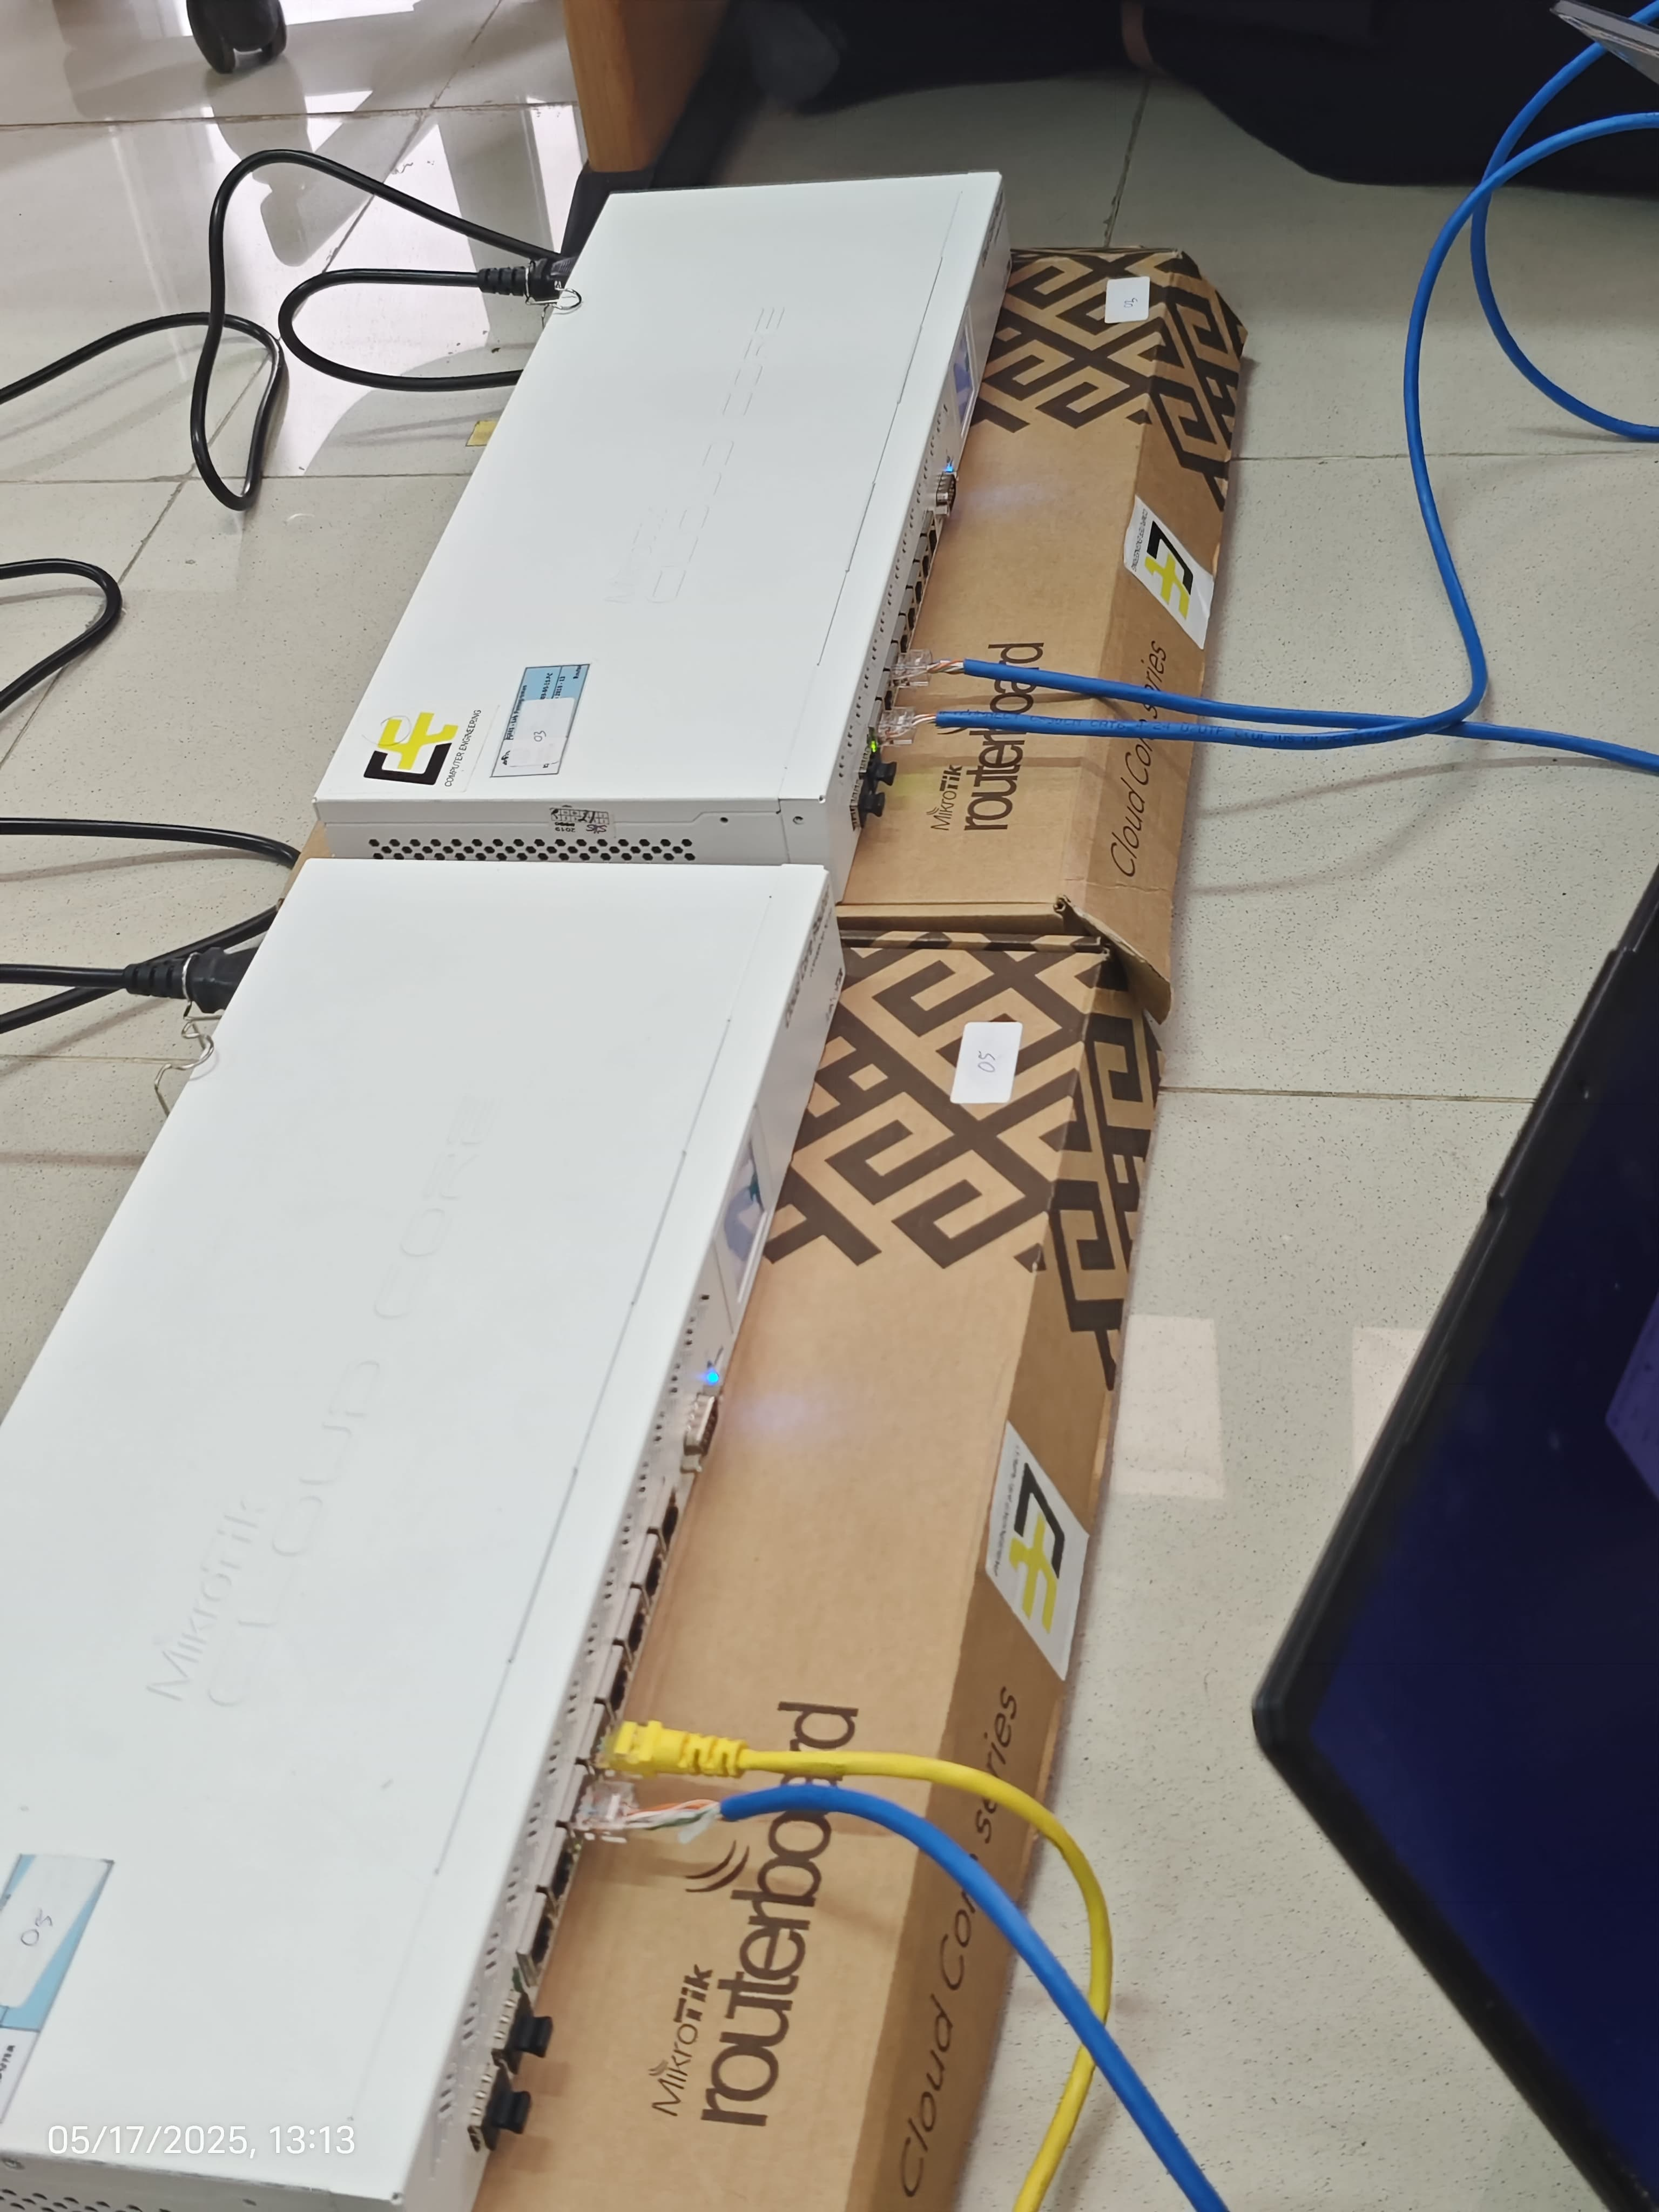
\includegraphics[width=0.48\textwidth]{img/Pasang.jpeg}
    \caption{Pemasangan kabel}
    \label{fig:pasang}
\end{figure}

Setelah terhubung secara fisik, buka Winbox untuk konfigurasi router.

\begin{figure}[H]
    \centering
    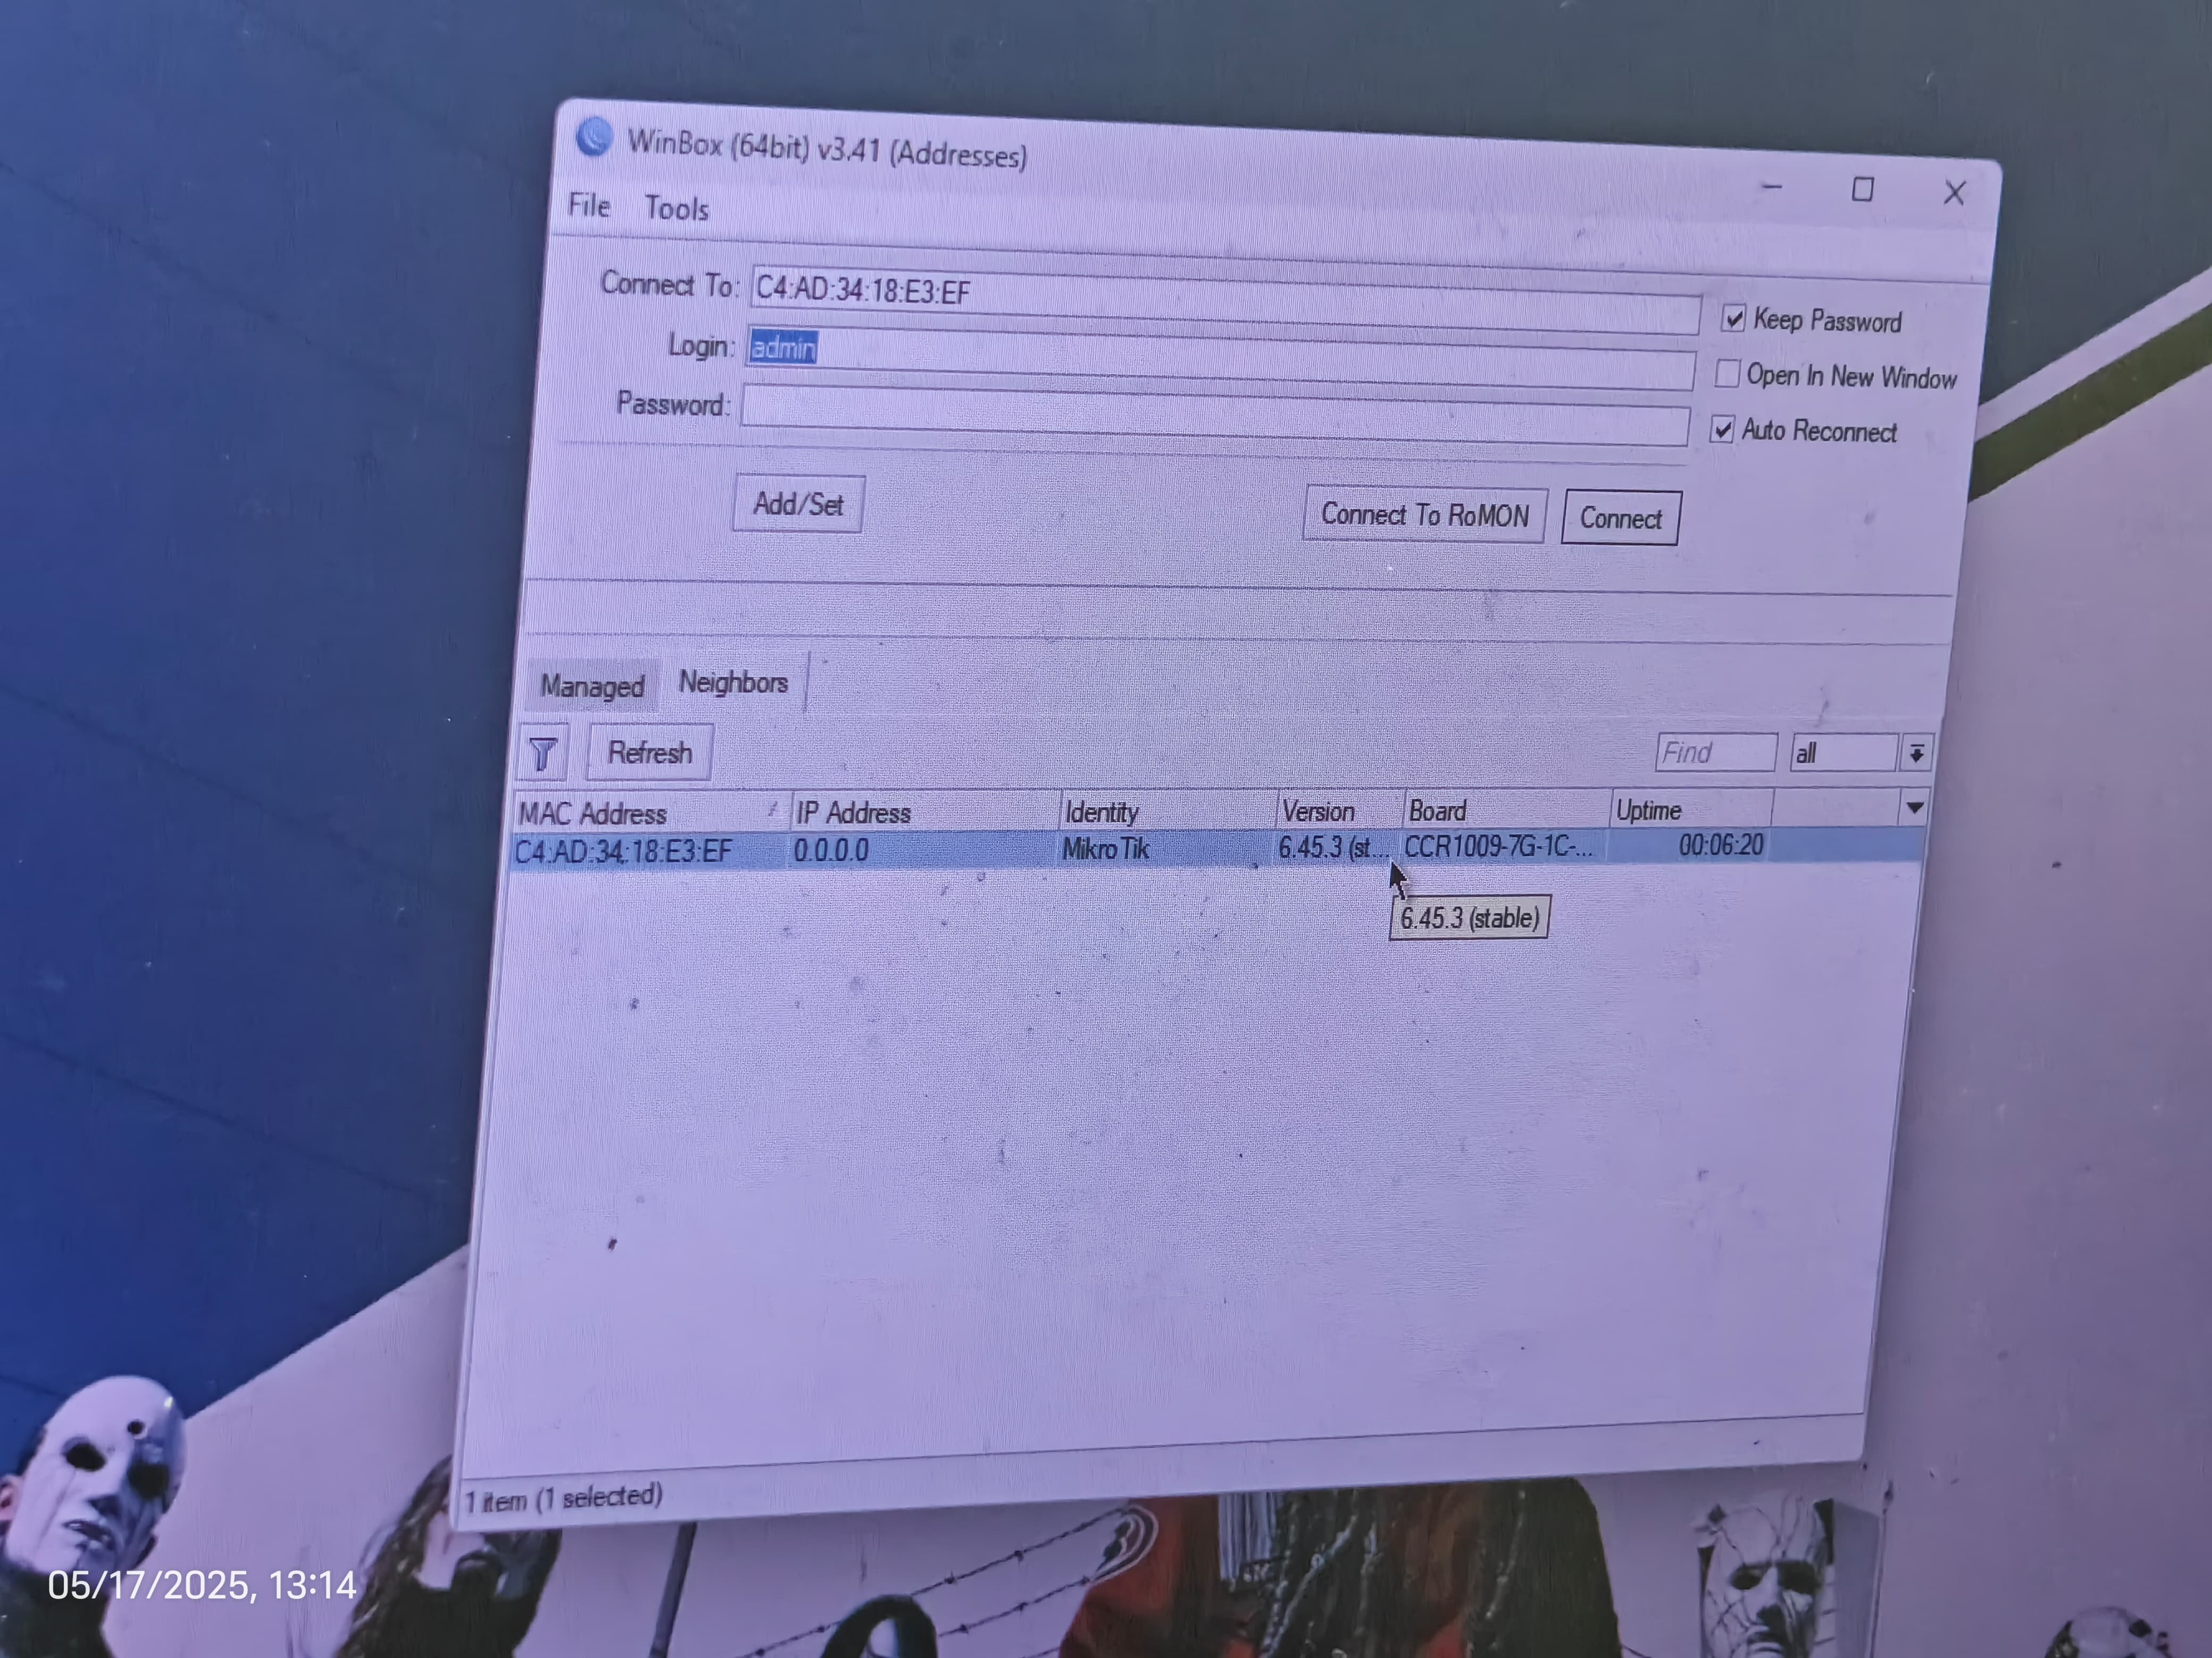
\includegraphics[width=0.48\textwidth]{img/winbox.jpeg}
    \caption{Masuk Winbox untuk konfigurasi router}
    \label{fig:winbox}
\end{figure}

Selanjutnya, pastikan setiap \textit{end device} telah terdaftar \textit{address}-nya.

\begin{figure}[H]
    \centering
    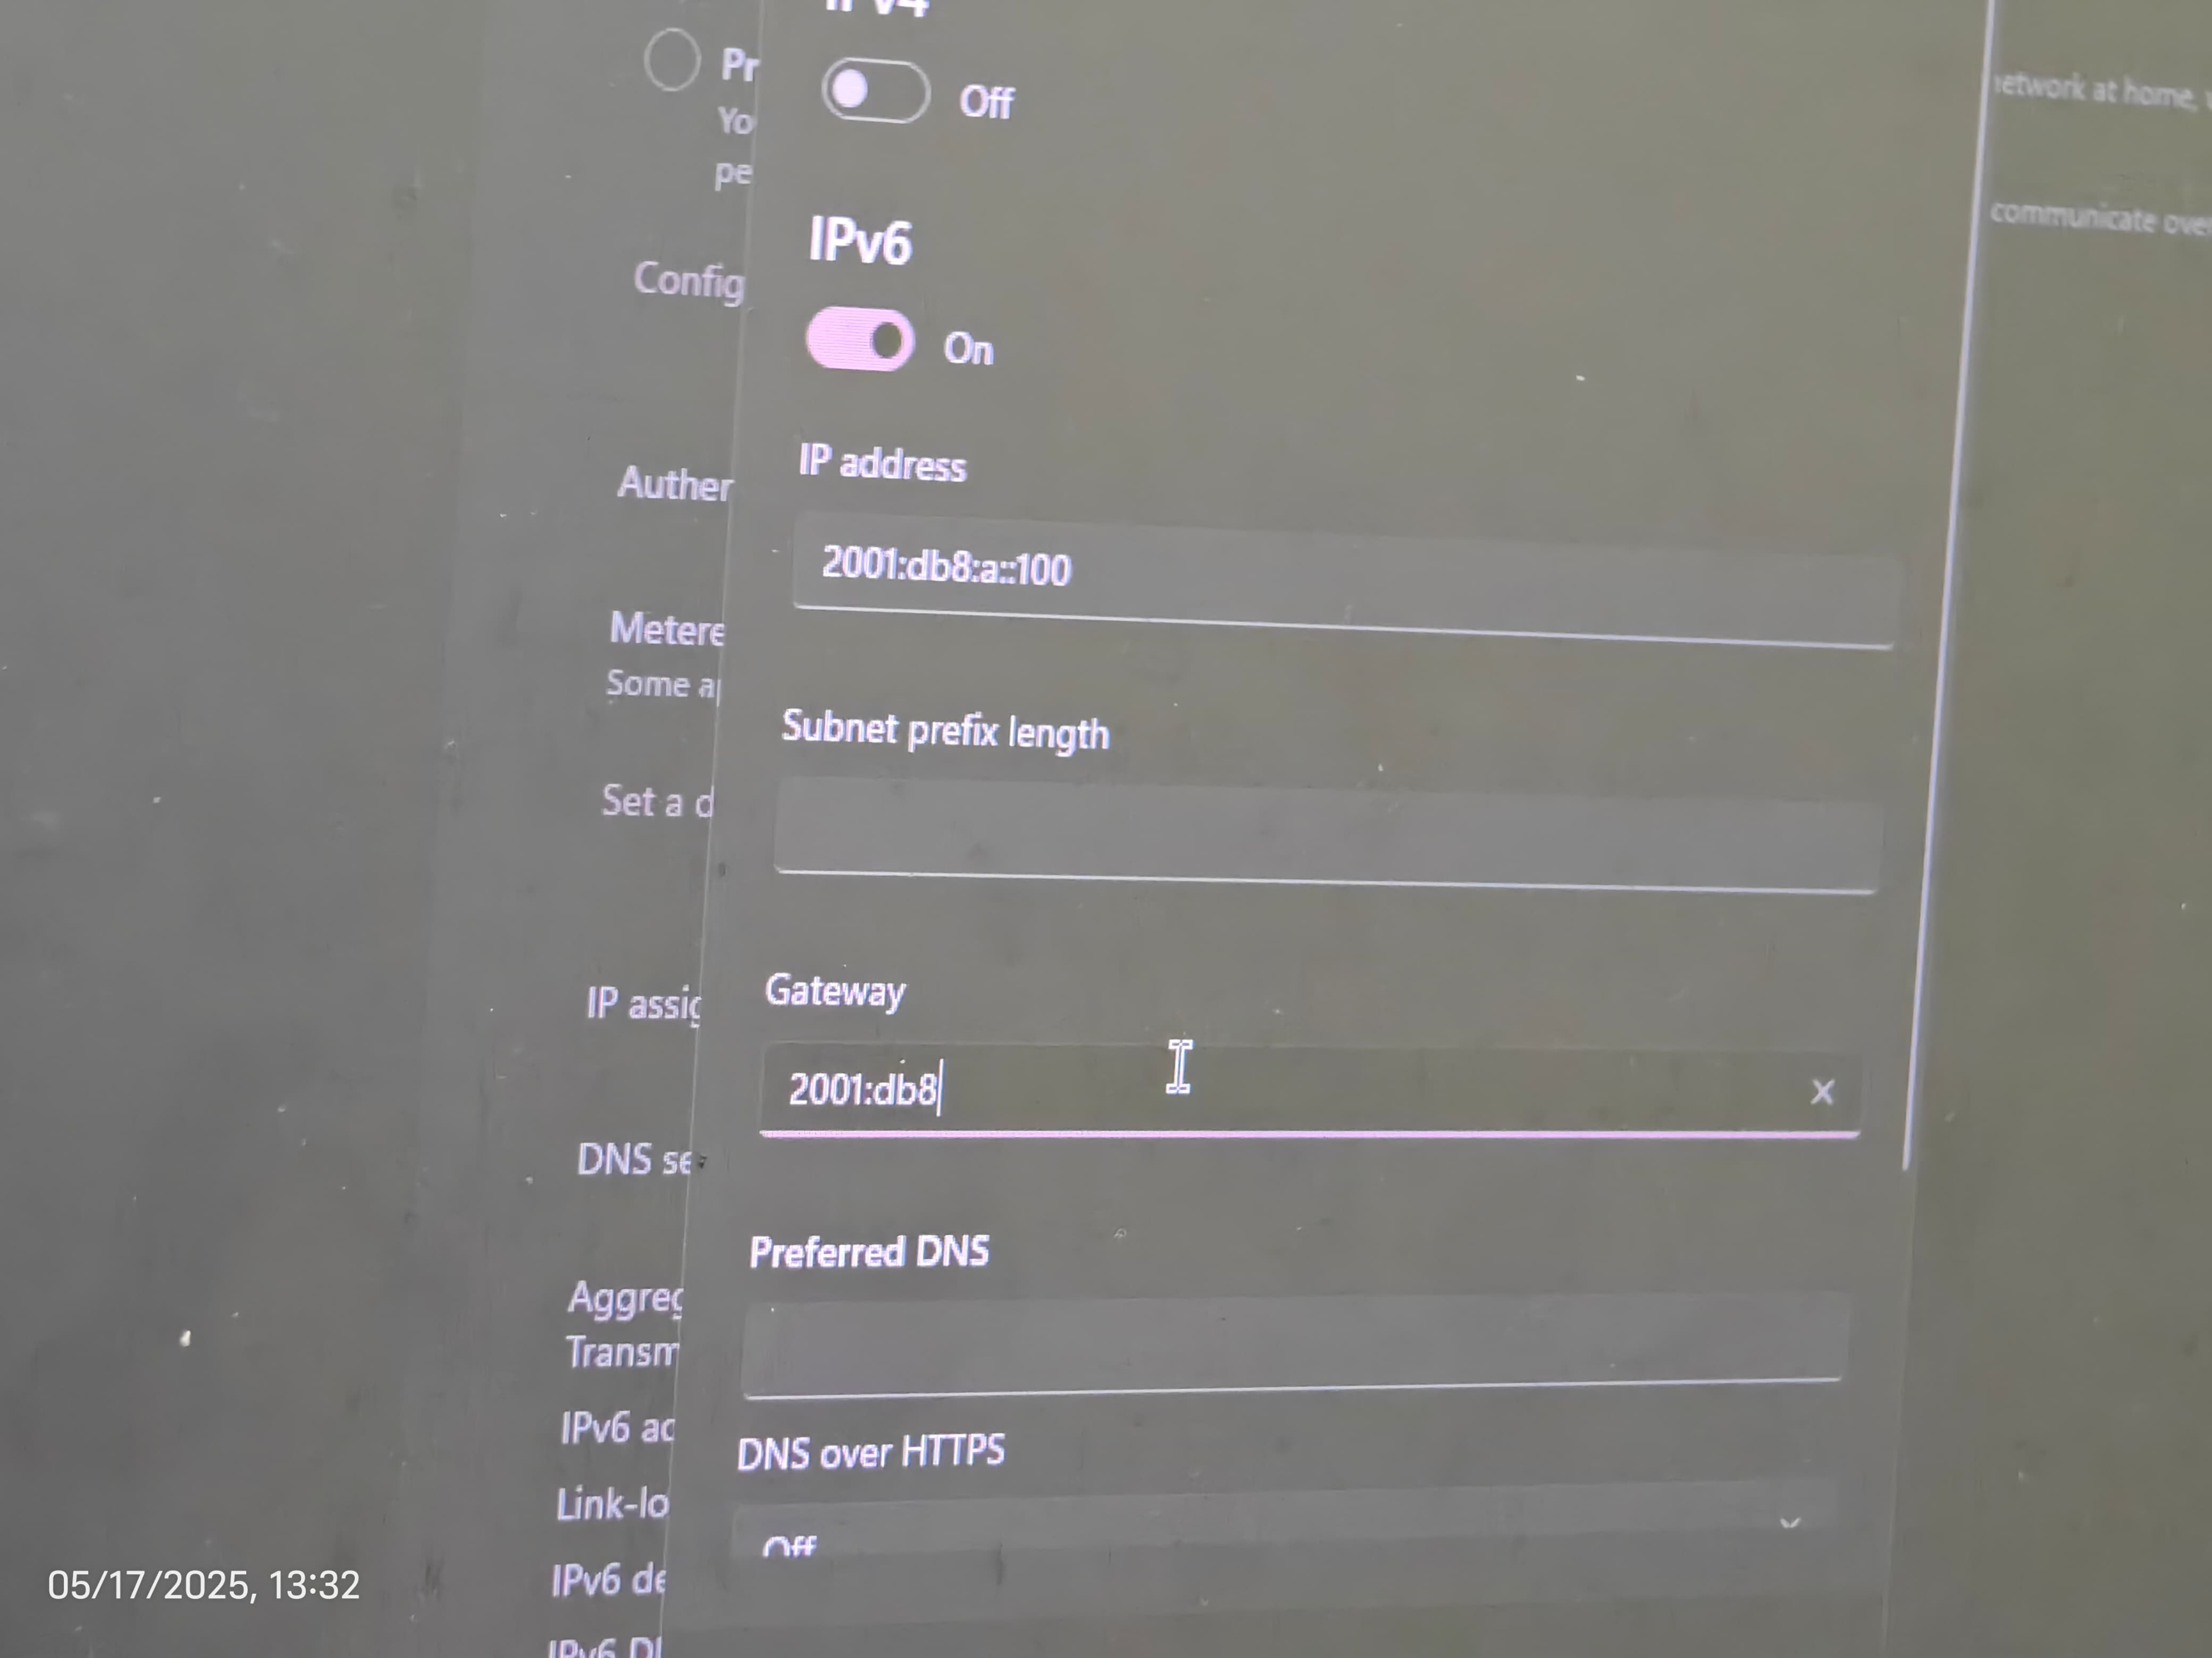
\includegraphics[width=0.48\textwidth]{img/address.jpeg}
    \caption{Address \textit{End Device}}
    \label{fig:address}
\end{figure}

Berikut konfigurasi \textit{address} untuk \textit{routing statis} IPv6. Tiga \textit{address} berikut ditujukan bagi Router\,1, Router\,2, dan PC2 (dengan asumsi \textit{end device} yang digunakan adalah PC1).

\begin{figure}[H]
    \centering
    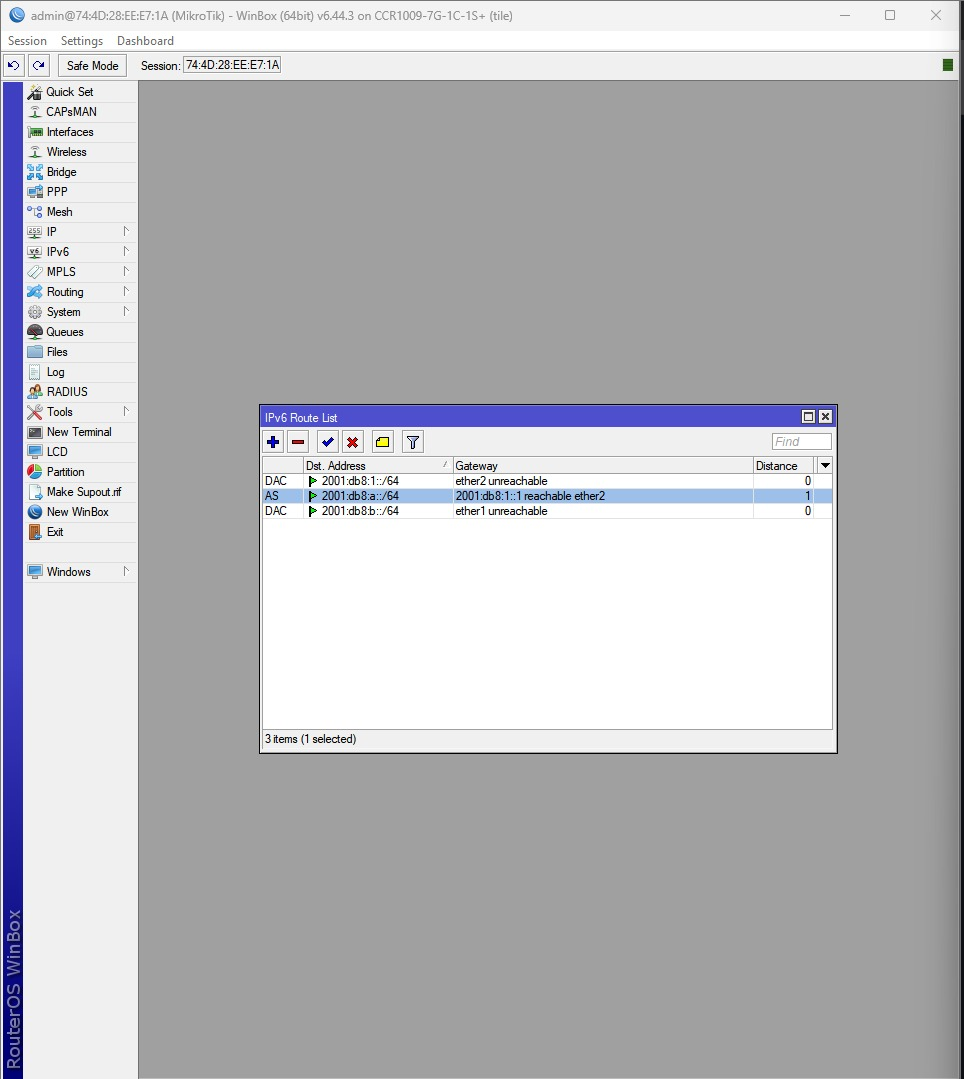
\includegraphics[width=0.48\textwidth]{img/A1.jpeg}
    \caption{Konfigurasi alamat}
    \label{fig:a1}
\end{figure}

Untuk memastikan koneksi telah terbangun, lakukan uji \textit{ping} dari kedua \textit{end device}.

\begin{figure}[H]
    \centering
    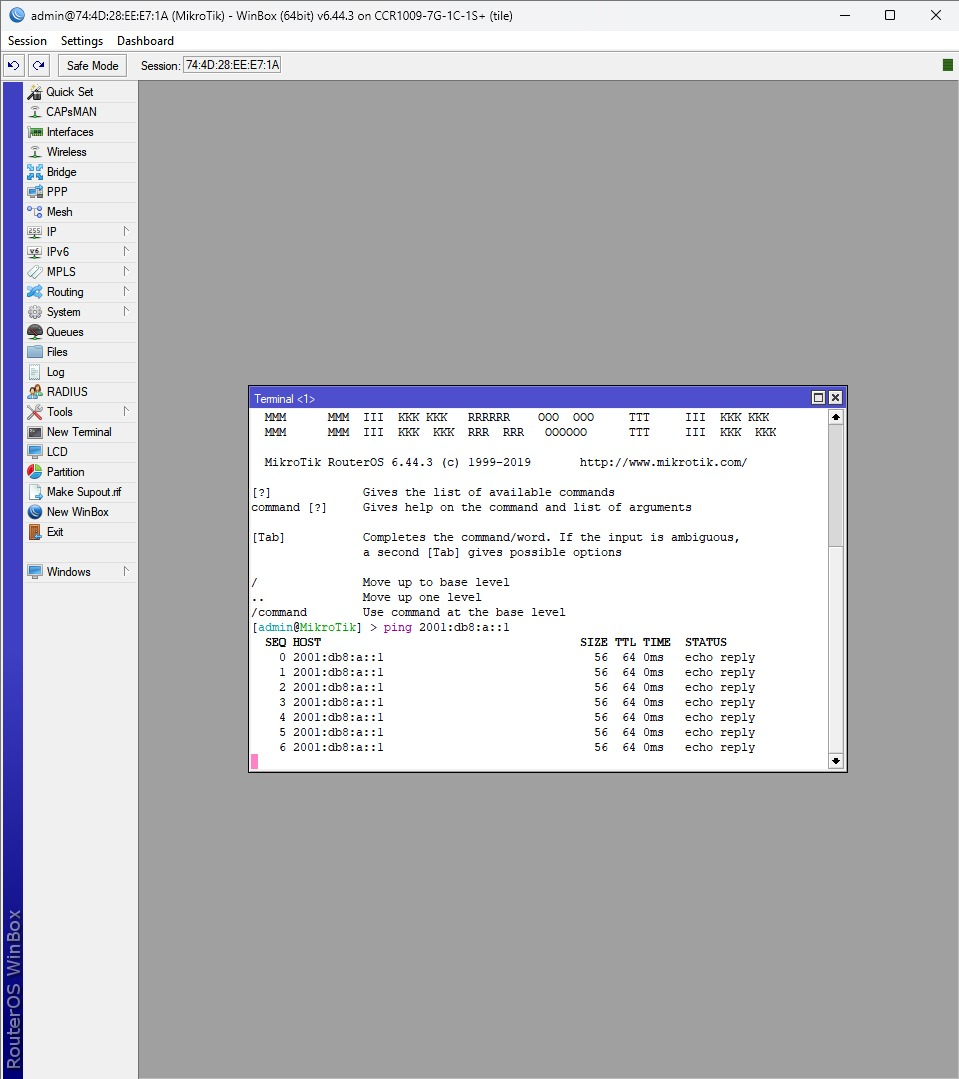
\includegraphics[width=0.48\textwidth]{img/A2.jpeg}
    \caption{Uji \textit{ping} dari PC1}
    \label{fig:a2a}
\end{figure}

\begin{figure}[H]
    \centering
    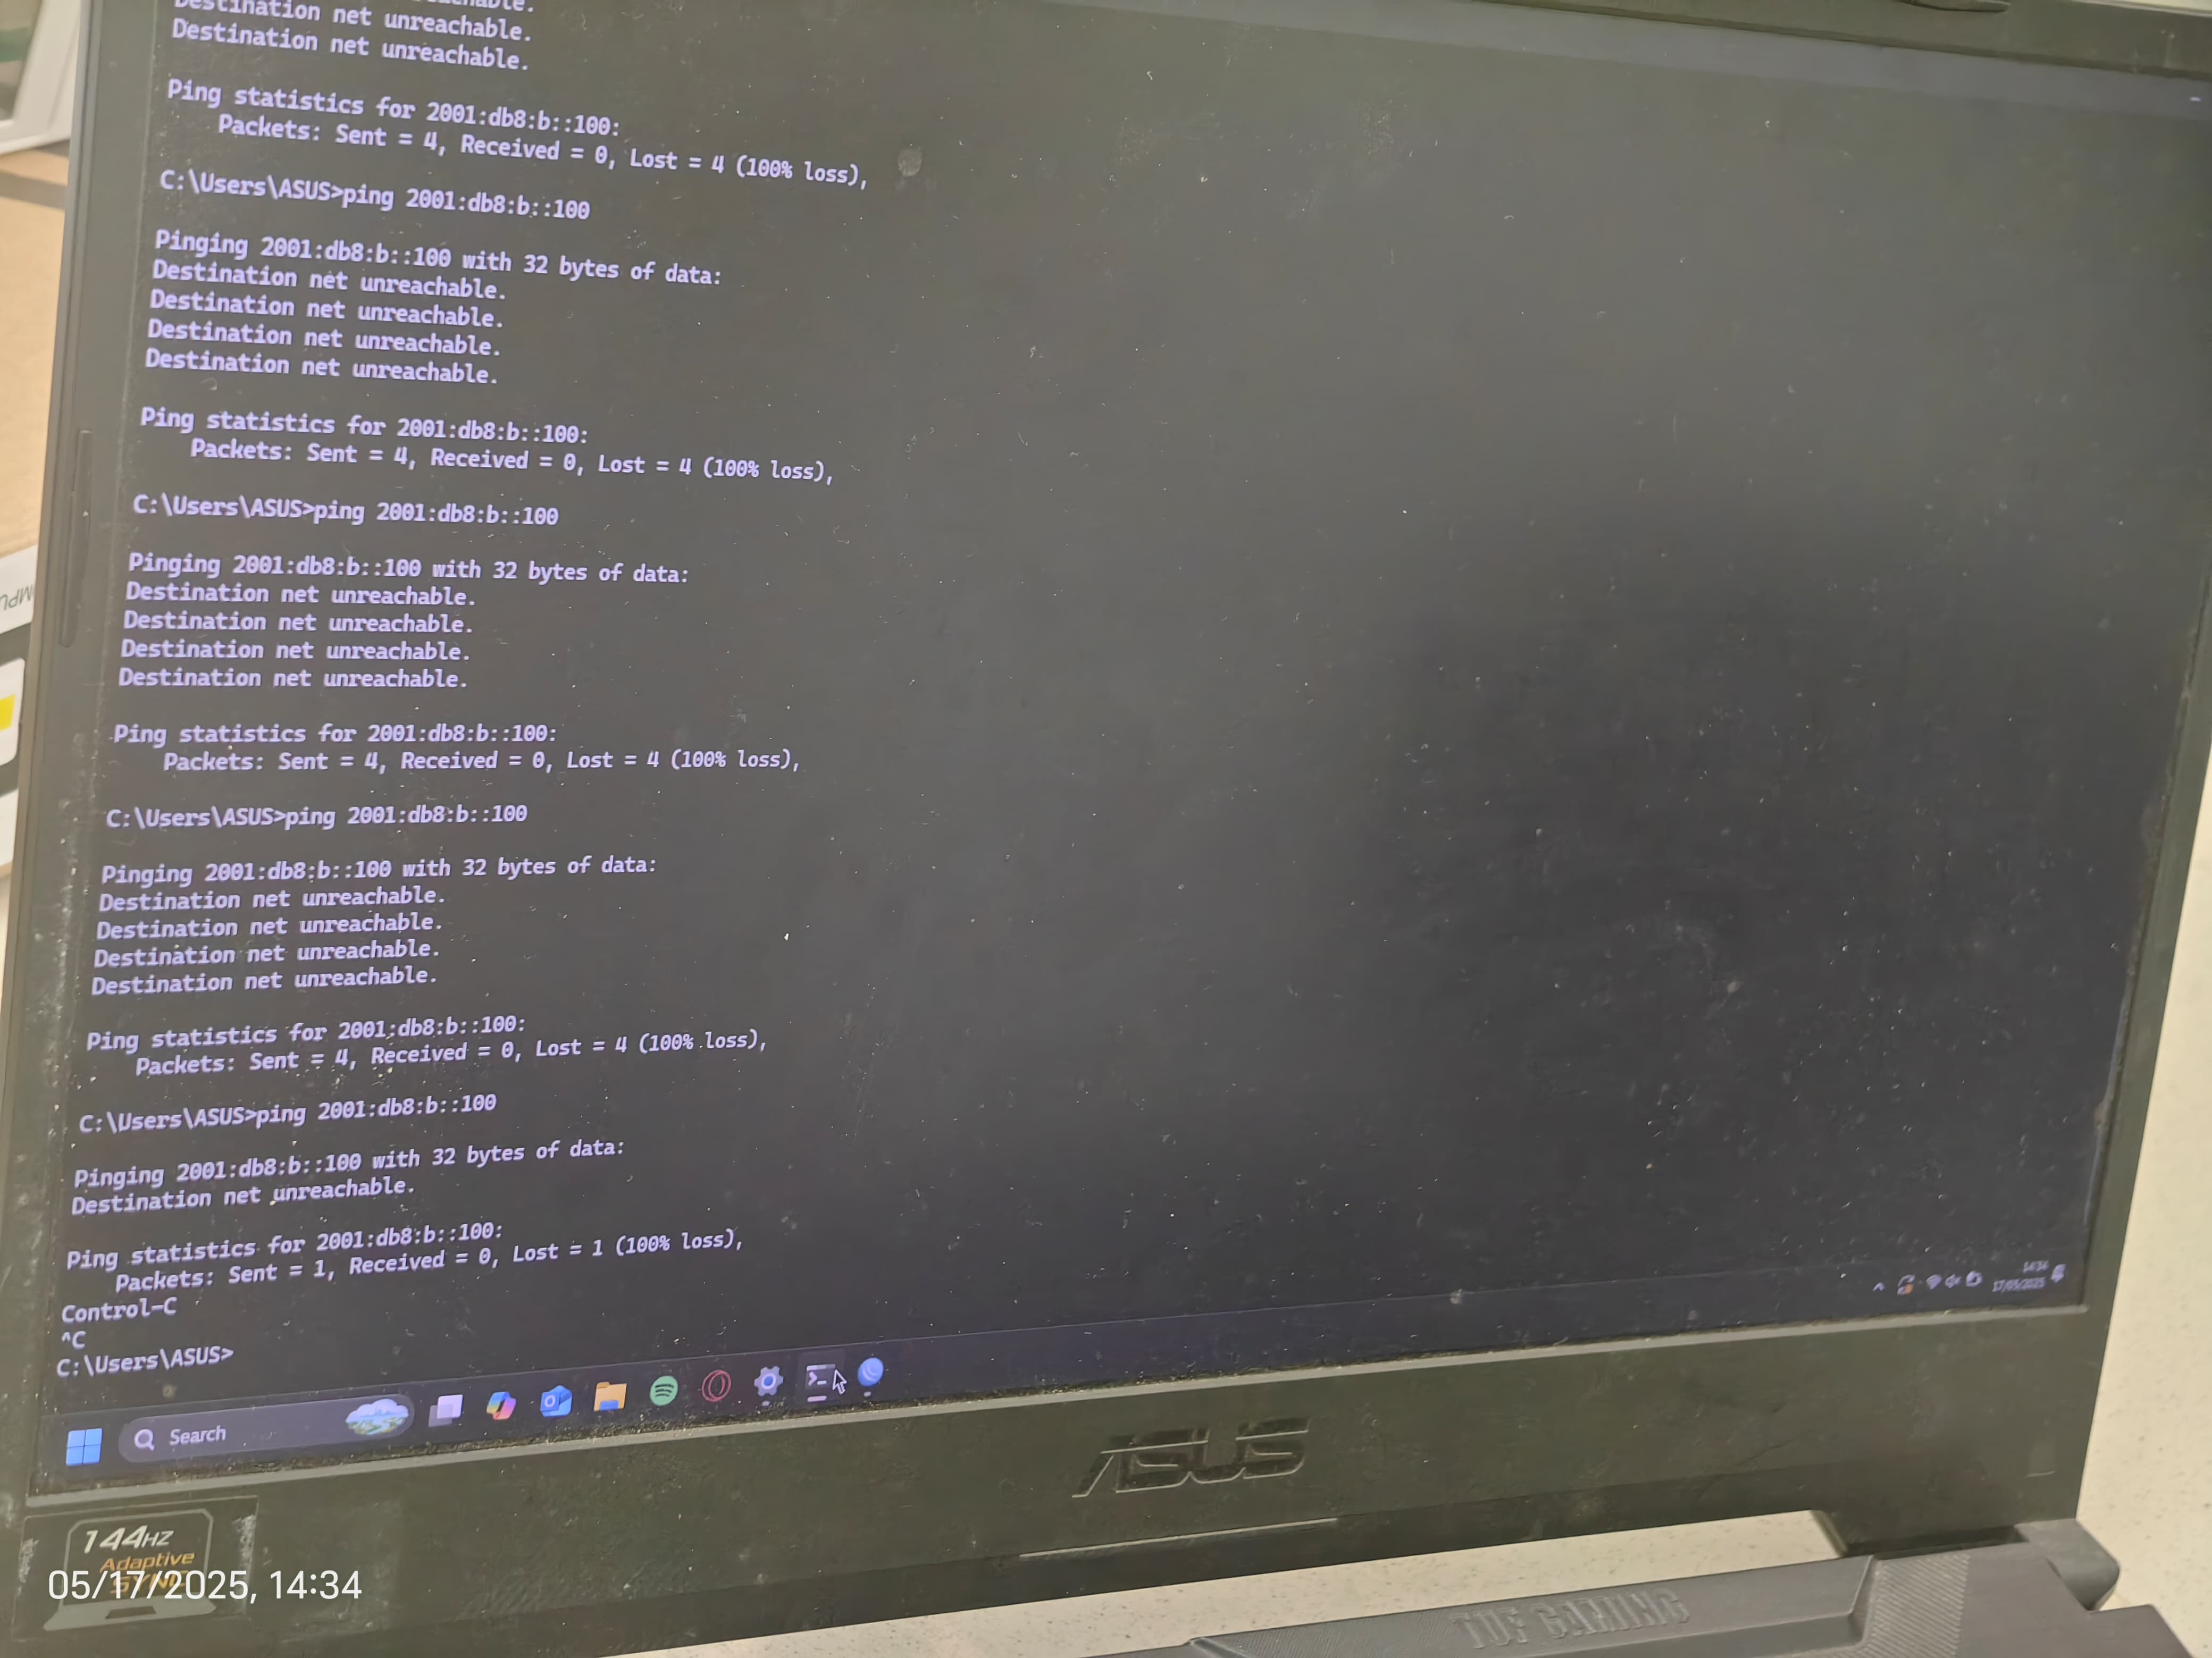
\includegraphics[width=0.48\textwidth]{img/A2-2.jpeg}
    \caption{Uji \textit{ping} dari PC2}
    \label{fig:a2b}
\end{figure}

\newpage

Setelah konfigurasi \textit{address} statis berhasil, dilanjutkan dengan uji coba \textit{routing dinamis}. Tiga \textit{address} berikut adalah milik Router\,2, PC1, dan Router\,1 (dengan asumsi \textit{end device} adalah PC2).

\begin{figure}[H]
    \centering
    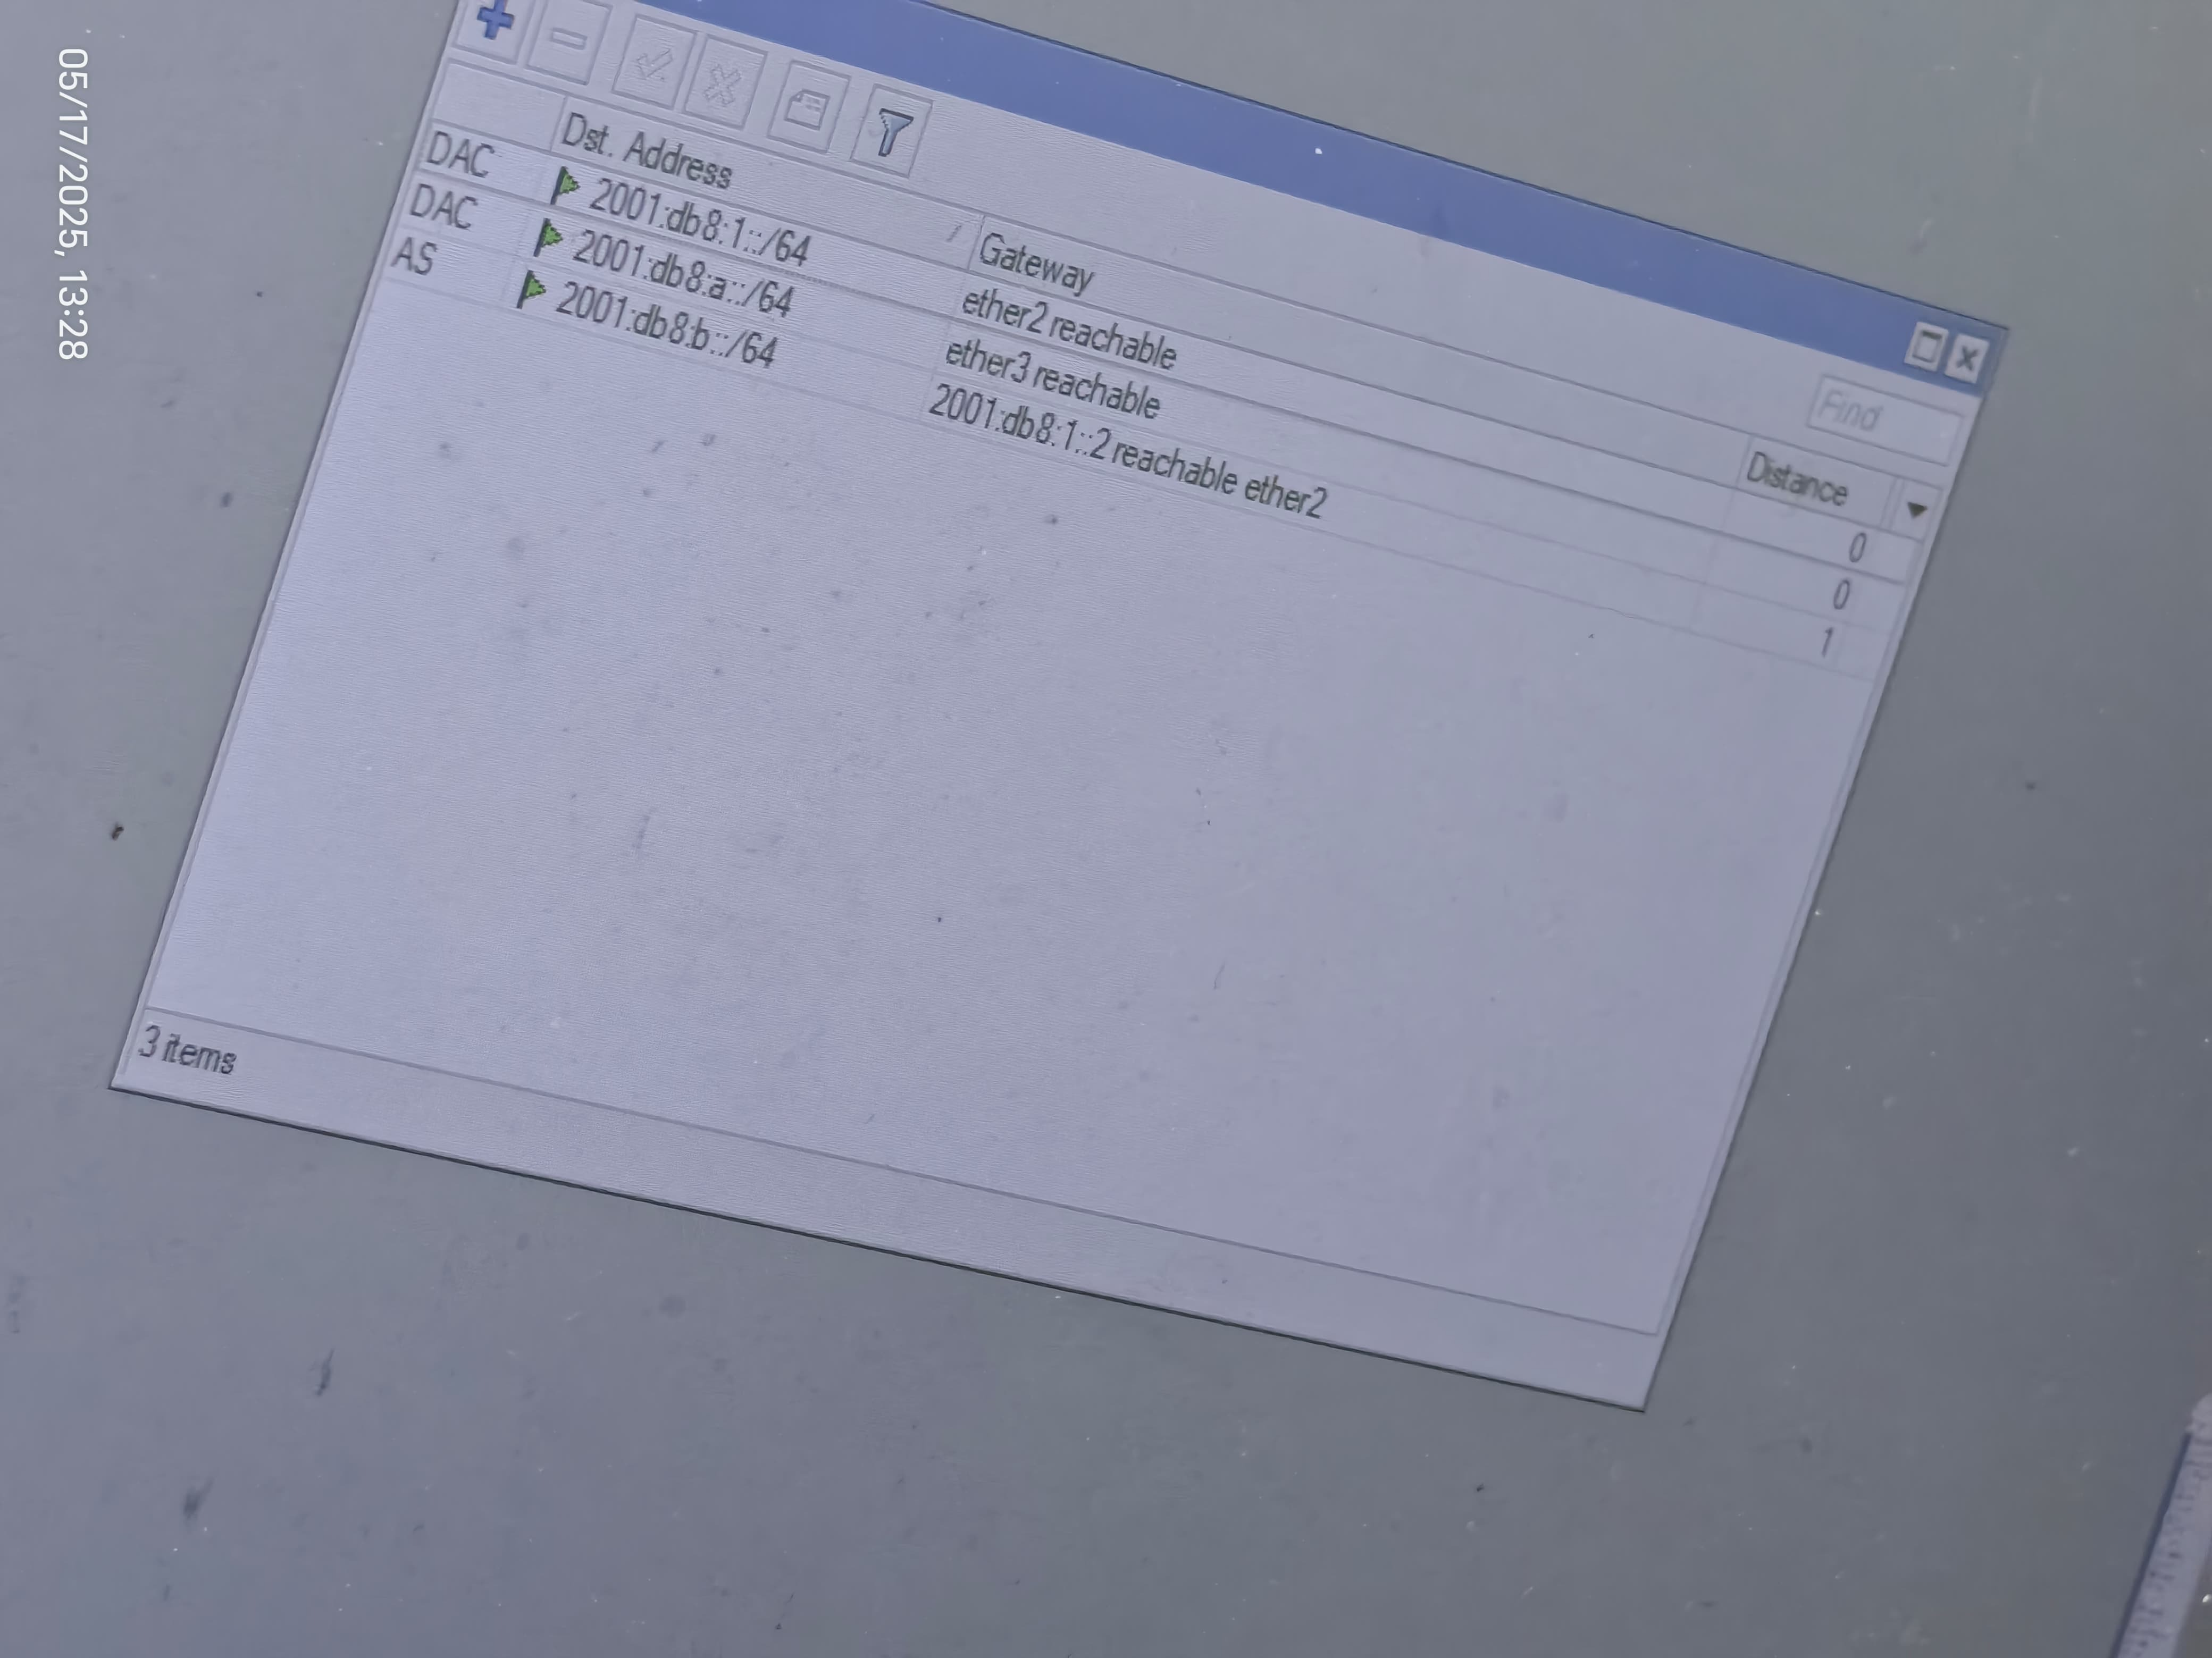
\includegraphics[width=0.48\textwidth]{img/A4.jpg}
    \caption{Konfigurasi alamat pada PC2}
    \label{fig:a4}
\end{figure}

\begin{figure}[H]
    \centering
    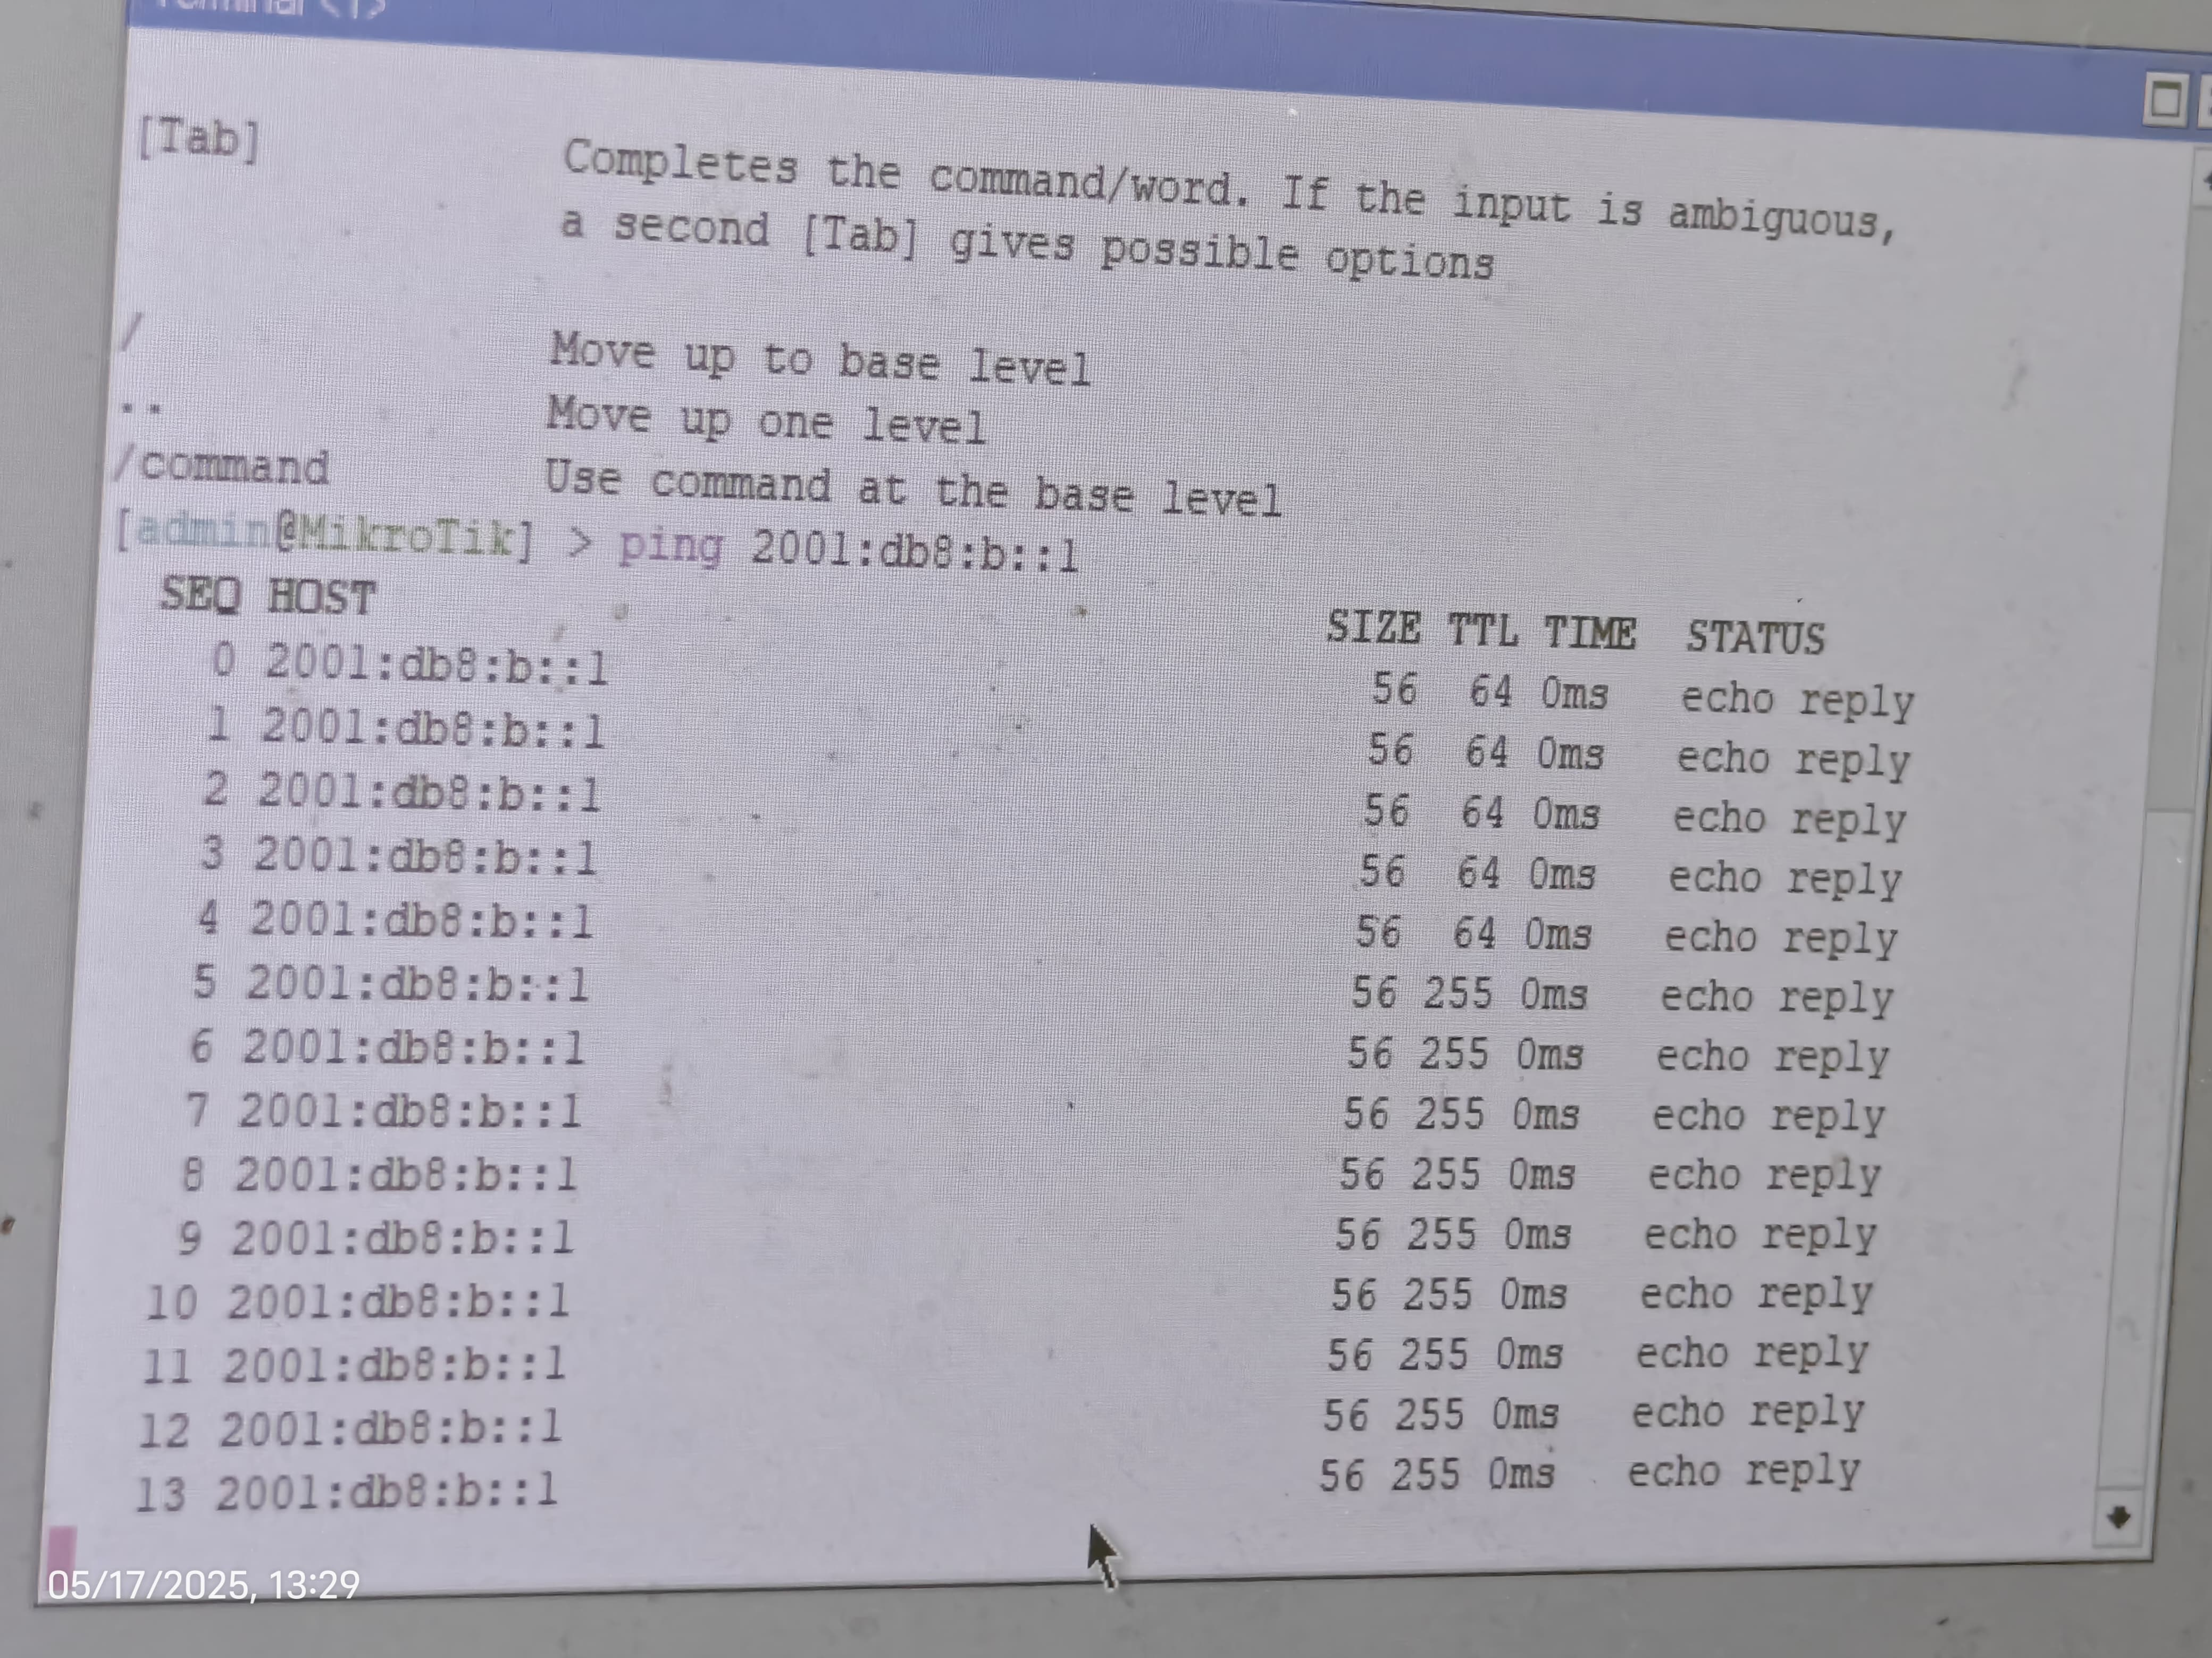
\includegraphics[width=0.48\textwidth]{img/A5.jpeg}
    \caption{Uji \textit{ping} pada PC2}
    \label{fig:a5}
\end{figure}

Konfigurasi OSPFv3 diterapkan pada kedua router agar secara otomatis saling bertukar informasi rute.

\begin{figure}[H]
    \centering
    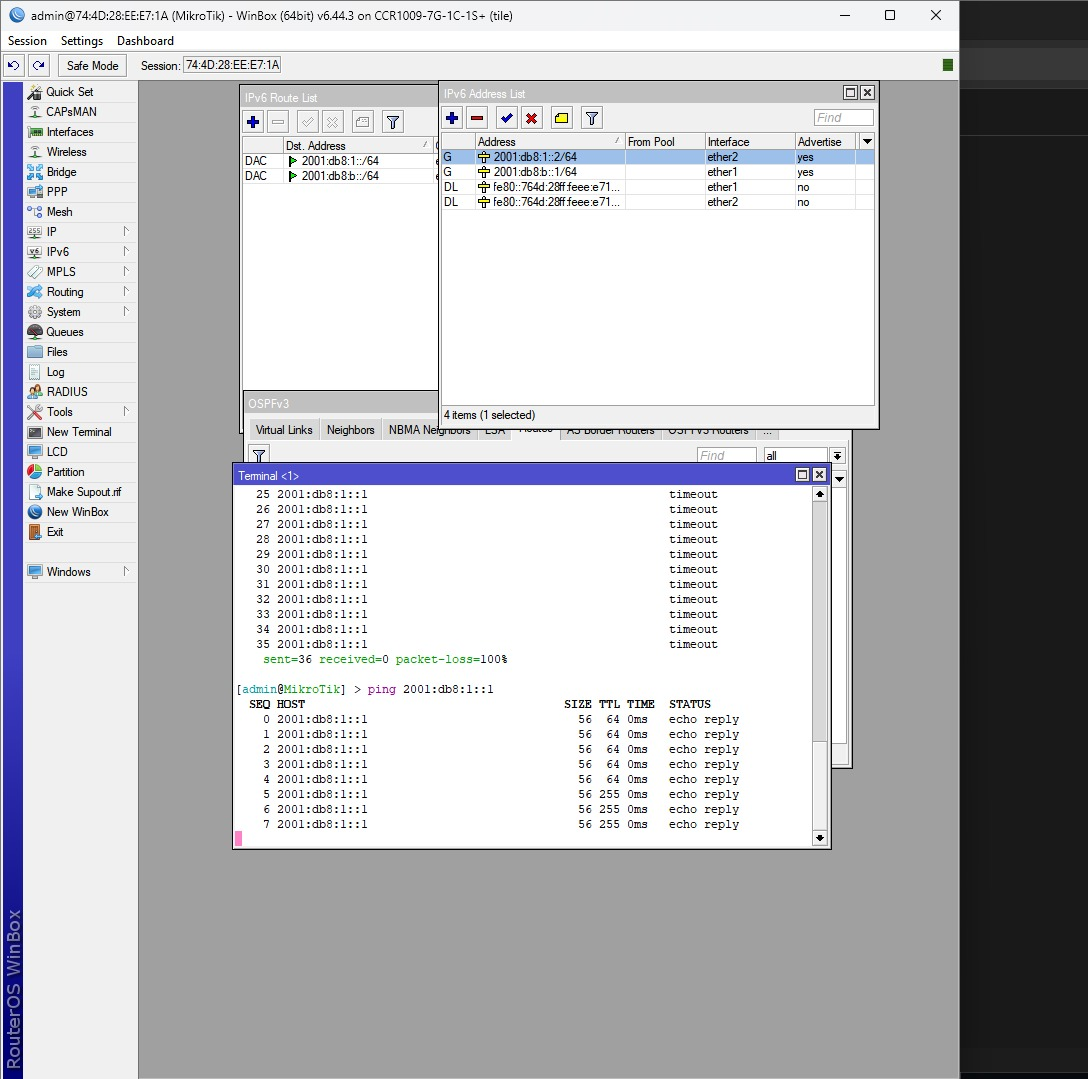
\includegraphics[width=0.48\textwidth]{img/A3.jpeg}
    \caption{Konfigurasi dan uji \textit{ping} pada PC1}
    \label{fig:a3}
\end{figure}

\newpage
\section{Analisis Hasil Percobaan}

\subsection{Routing Statis IPv6}

Router diinisialisasi ulang untuk menghindari konflik konfigurasi lama. IP pada \textit{interface} antarr­outer (Ether1) disetel ke
\texttt{2001:db8:1::1/64} (Router\,1) dan \texttt{2001:db8:1::2/64} (Router\,2). Pada jaringan LAN,
Ether2 Router\,1 menggunakan \texttt{2001:db8:a::1/64} dan Ether2 Router\,2 menggunakan \texttt{2001:db8:b::1/64}.

Rute statis ditambahkan:
\begin{itemize}
    \item Router\,1: tujuan \texttt{2001:db8:b::/64}, \textit{gateway} \texttt{2001:db8:1::2}
    \item Router\,2: tujuan \texttt{2001:db8:a::/64}, \textit{gateway} \texttt{2001:db8:1::1}
\end{itemize}

Tes \textit{ping} berhasil antara kedua router dan kedua laptop (IP laptop: \texttt{2001:db8:a::100/64} dan \texttt{2001:db8:b::100/64}), menandakan \textit{routing statis} berjalan tanpa kendala.

\subsection{Routing Dinamis IPv6}

Selanjutnya OSPFv3 dikonfigurasi. \textit{Router ID} ditetapkan menjadi \texttt{1.1.1.1} (Router\,1) dan \texttt{2.2.2.2} (Router\,2) dengan \texttt{Area ID 0.0.0.0}. Setelah status \textit{Neighbor} OSPF terpantau aktif, tes \textit{ping} antarr­outer dan antar-laptop berhasil, membuktikan \textit{routing dinamis} IPv6 berfungsi sebagaimana mestinya.

\newpage
\section{Hasil Tugas Modul}

Tugas modul mensyaratkan demonstrasi \textit{routing statis} dan \textit{routing dinamis} IPv6 menggunakan Cisco Packet Tracer.

\subsection{Routing Statis}

Topologi jaringan statis:

\begin{figure}[H]
    \centering
    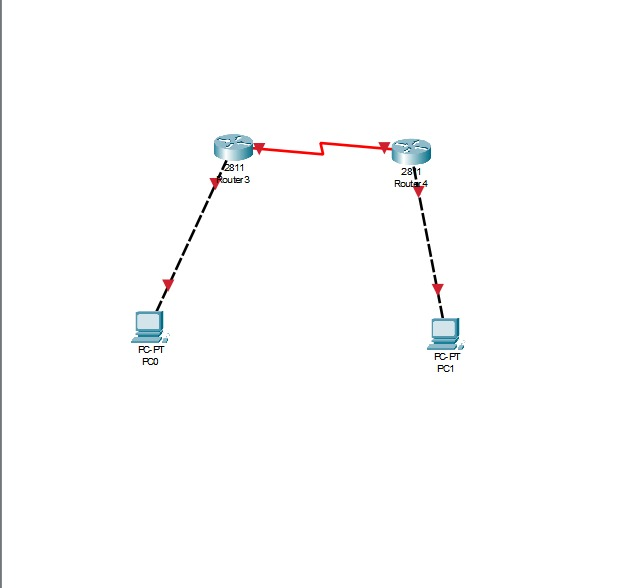
\includegraphics[width=0.48\textwidth]{img/TM1.jpeg}
    \caption{Topologi sebelum terkoneksi}
    \label{fig:tm1}
\end{figure}

Konfigurasi IP \textit{end device}:
\begin{itemize}
    \item \textbf{PC0}
        \begin{itemize}
            \item IPv6: \texttt{2001:DB8:1:1::2/64}
            \item Link-local: \texttt{FE80::260:3EFF:FE2D:DC50}
            \item Default GW: \texttt{2001:DB8:1:1::1}
        \end{itemize}
    \item \textbf{PC1}
        \begin{itemize}
            \item IPv6: \texttt{2001:DB8:1:2::2/64}
            \item Link-local: \texttt{FE80::2D0:97FF:FE61:187B}
            \item Default GW: \texttt{2001:DB8:1:2::1}
        \end{itemize}
\end{itemize}

\begin{figure}[H]
    \centering
    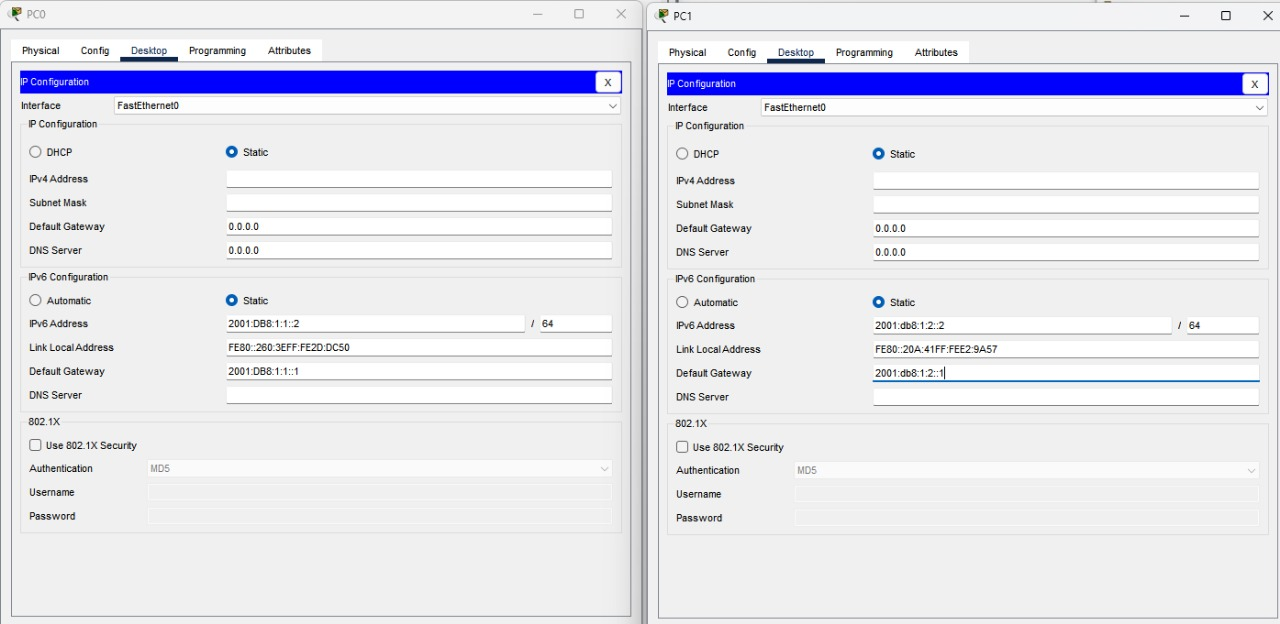
\includegraphics[width=0.48\textwidth]{img/TM2.jpeg}
    \caption{Konfigurasi alamat kedua \textit{end device}}
    \label{fig:tm2}
\end{figure}

\paragraph{Cuplikan CLI Router\,3}
\begin{verbatim}
Router 3 CLI Output:
%LINEPROTO-5-UPDOWN: Line protocol on Interface FastEthernet0/0, changed state to up
%LINK-5-CHANGED: Interface Serial1/0, changed state to up
%LINEPROTO-5-UPDOWN: Line protocol on Interface Serial1/0, changed state to up
\end{verbatim}

\paragraph{Konfigurasi Routing Statis Router\,3}
\begin{verbatim}
ip route 2001:DB8:1:2::/64 2001:DB8:1:1::1
ip route 2001:DB8:1:1::/64 2001:DB8:1:2::1
\end{verbatim}

Pengujian \textit{ping} PC0-PC1 berhasil, menandakan konfigurasi statis IPv6 berfungsi.

\begin{figure}[H]
    \centering
    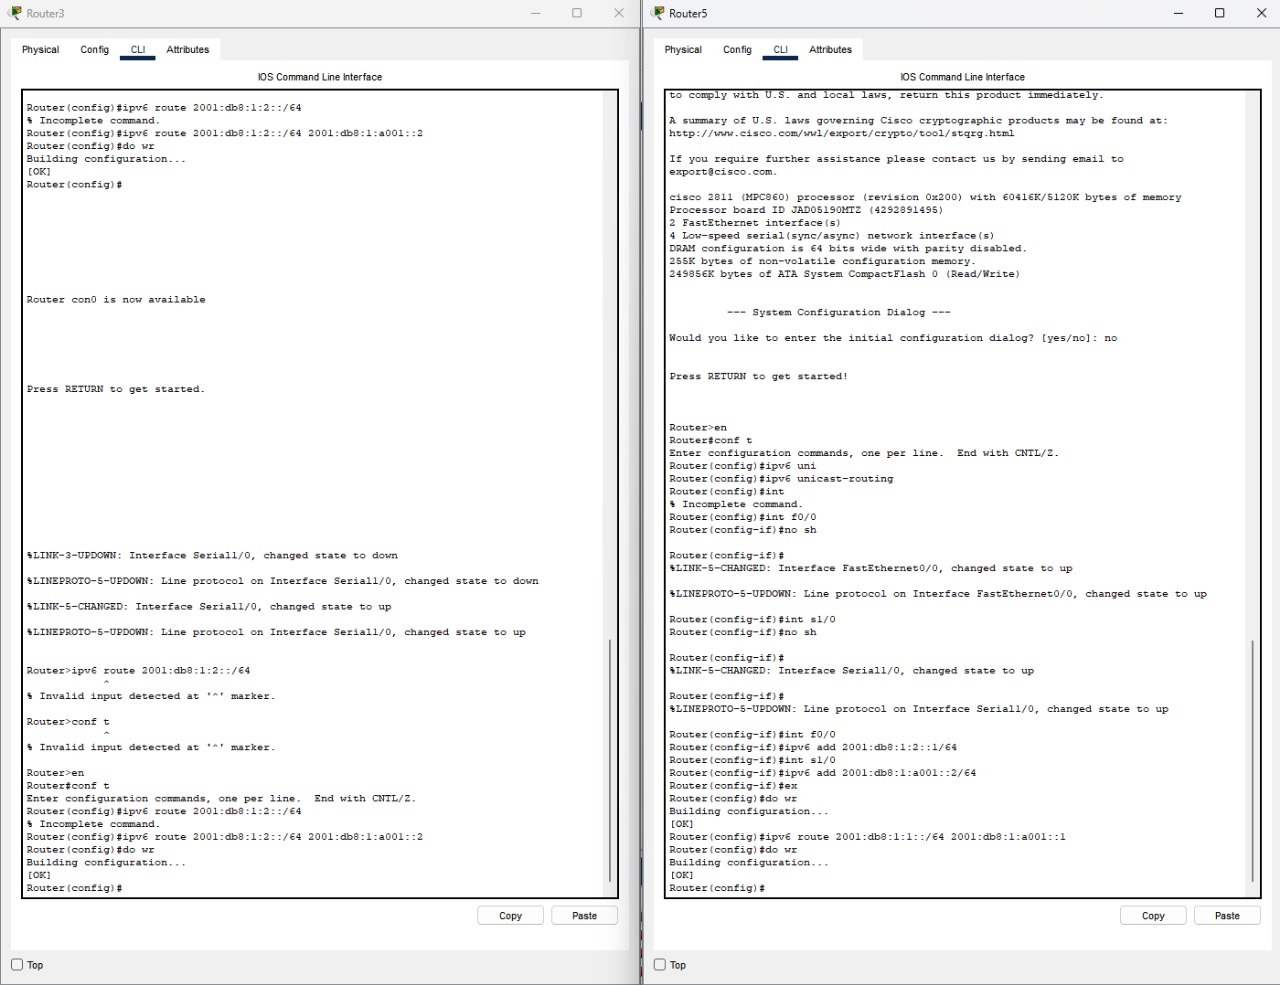
\includegraphics[width=0.48\textwidth]{img/TM3.jpeg}
    \caption{CLI konfigurasi antarr­outer}
    \label{fig:tm3}
\end{figure}

\begin{figure}[H]
    \centering
    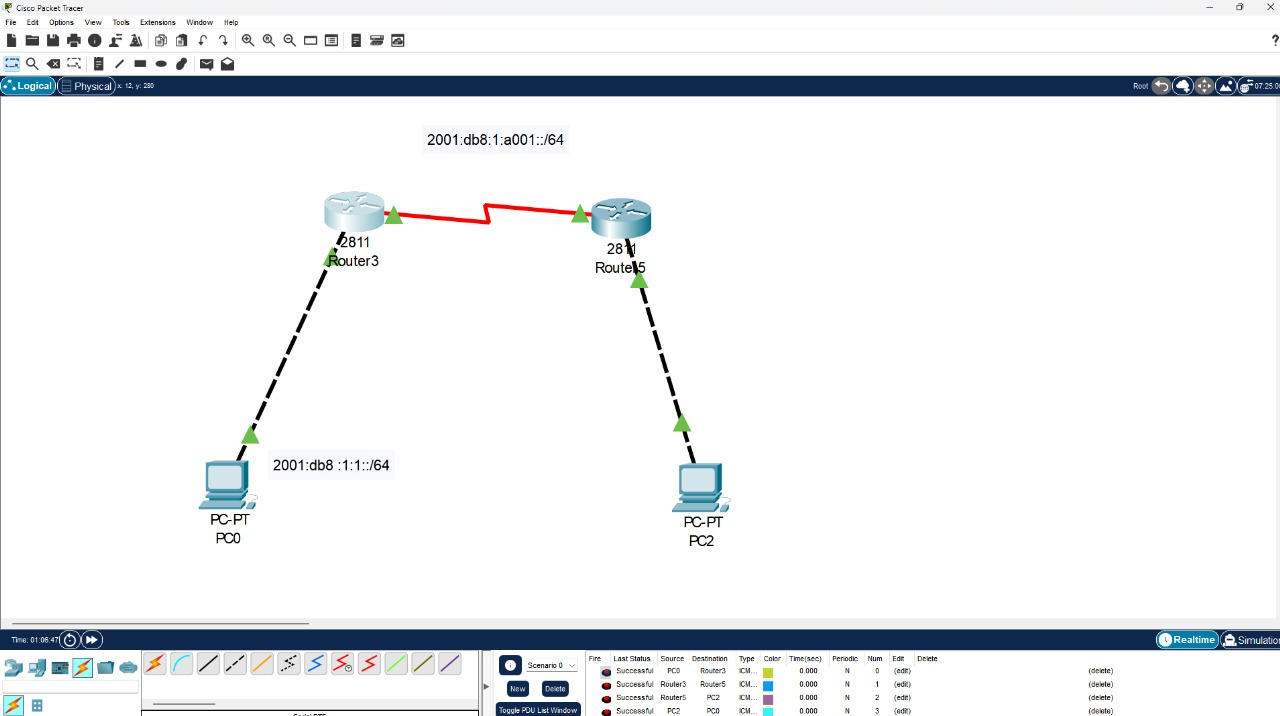
\includegraphics[width=0.48\textwidth]{img/TM4.jpeg}
    \caption{Topologi terkoneksi dan uji \textit{ping}}
    \label{fig:tm4}
\end{figure}

\newpage
\subsection{Routing Dinamis}

Topologi jaringan dinamis:

\begin{figure}[H]
    \centering
    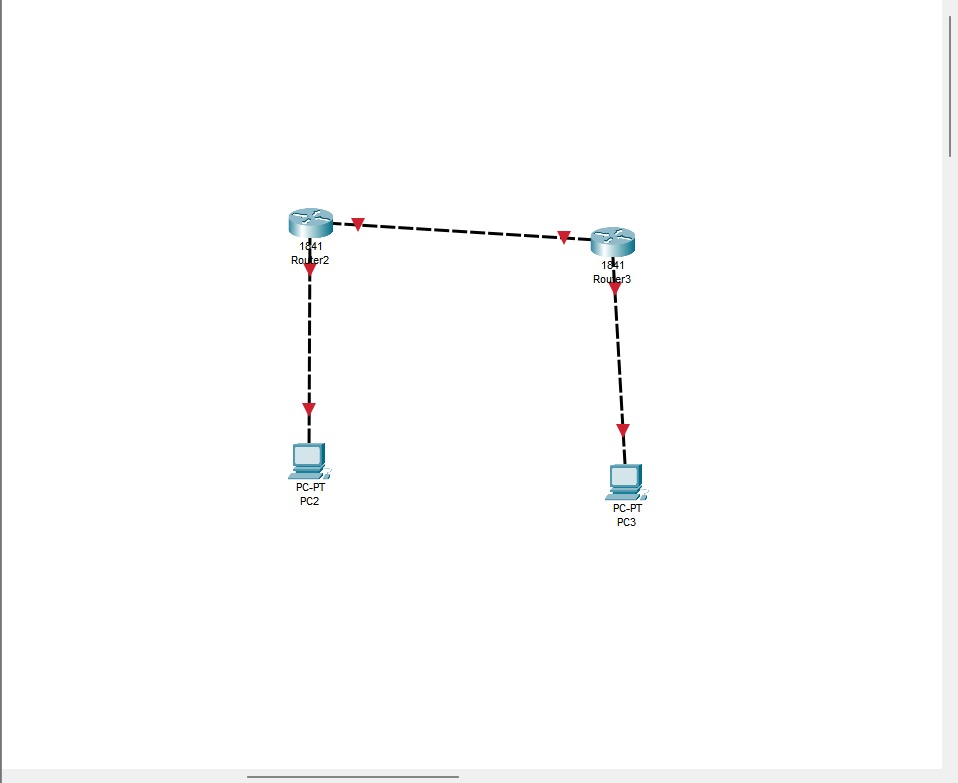
\includegraphics[width=0.48\textwidth]{img/TM5.jpeg}
    \caption{Topologi sebelum terkoneksi}
    \label{fig:tm5}
\end{figure}

Konfigurasi IP \textit{end device}:
\begin{itemize}
    \item \textbf{PC0}
        \begin{itemize}
            \item IPv6: \texttt{2007::1/64}
            \item Link-local: \texttt{FE80::250:FFF:FEEA:2988}
            \item Default GW: \texttt{2007::2}
        \end{itemize}
    \item \textbf{PC1}
        \begin{itemize}
            \item IPv6: \texttt{2009::1/64}
            \item Link-local: \texttt{FE80::20A:41FF:FED2:68A1}
            \item Default GW: \texttt{2009::2}
        \end{itemize}
\end{itemize}

\begin{figure}[H]
    \centering
    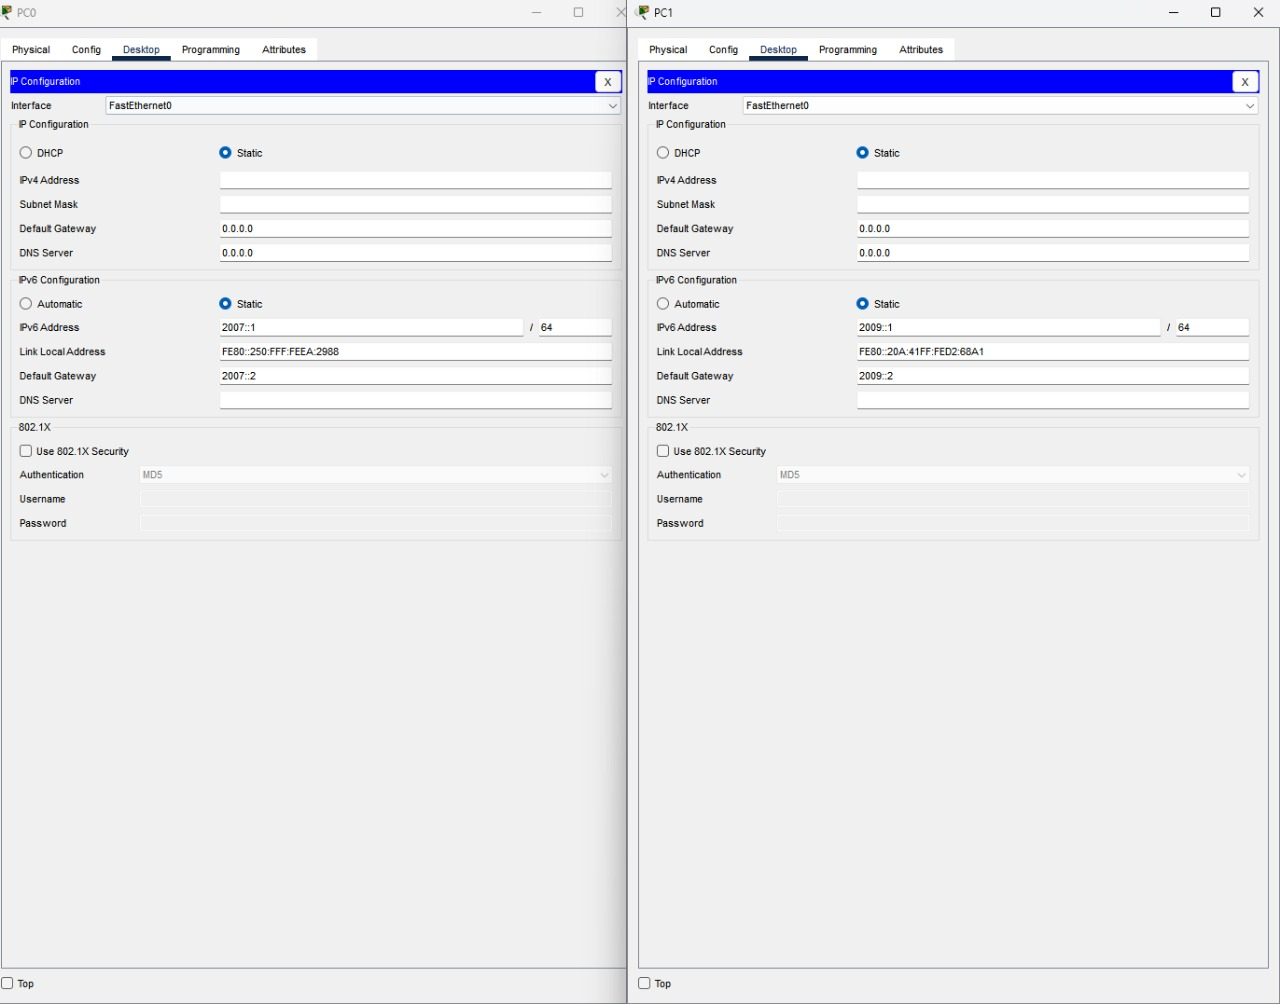
\includegraphics[width=0.48\textwidth]{img/TM6.jpeg}
    \caption{Konfigurasi alamat kedua \textit{end device}}
    \label{fig:tm6}
\end{figure}

\paragraph{Konfigurasi Router\,0}
\begin{verbatim}
ipv6 unicast-routing

interface fastethernet 0/1
 ipv6 address 2007::2/64
 ipv6 rip abc enable
 ipv6 enable
 no shut

interface fastethernet 0/0
 ipv6 address 2008::1/64
 ipv6 rip abc enable
 ipv6 enable
 no shut
\end{verbatim}

\paragraph{Konfigurasi Router\,1}
\begin{verbatim}
ipv6 unicast-routing

interface fastethernet 0/0
 ipv6 address 2008::2/64
 ipv6 rip abc enable
 ipv6 enable
 no shut

interface fastethernet 0/1
 ipv6 address 2009::2/64
 ipv6 rip abc enable
 ipv6 enable
 no shut
\end{verbatim}

\begin{figure}[H]
    \centering
    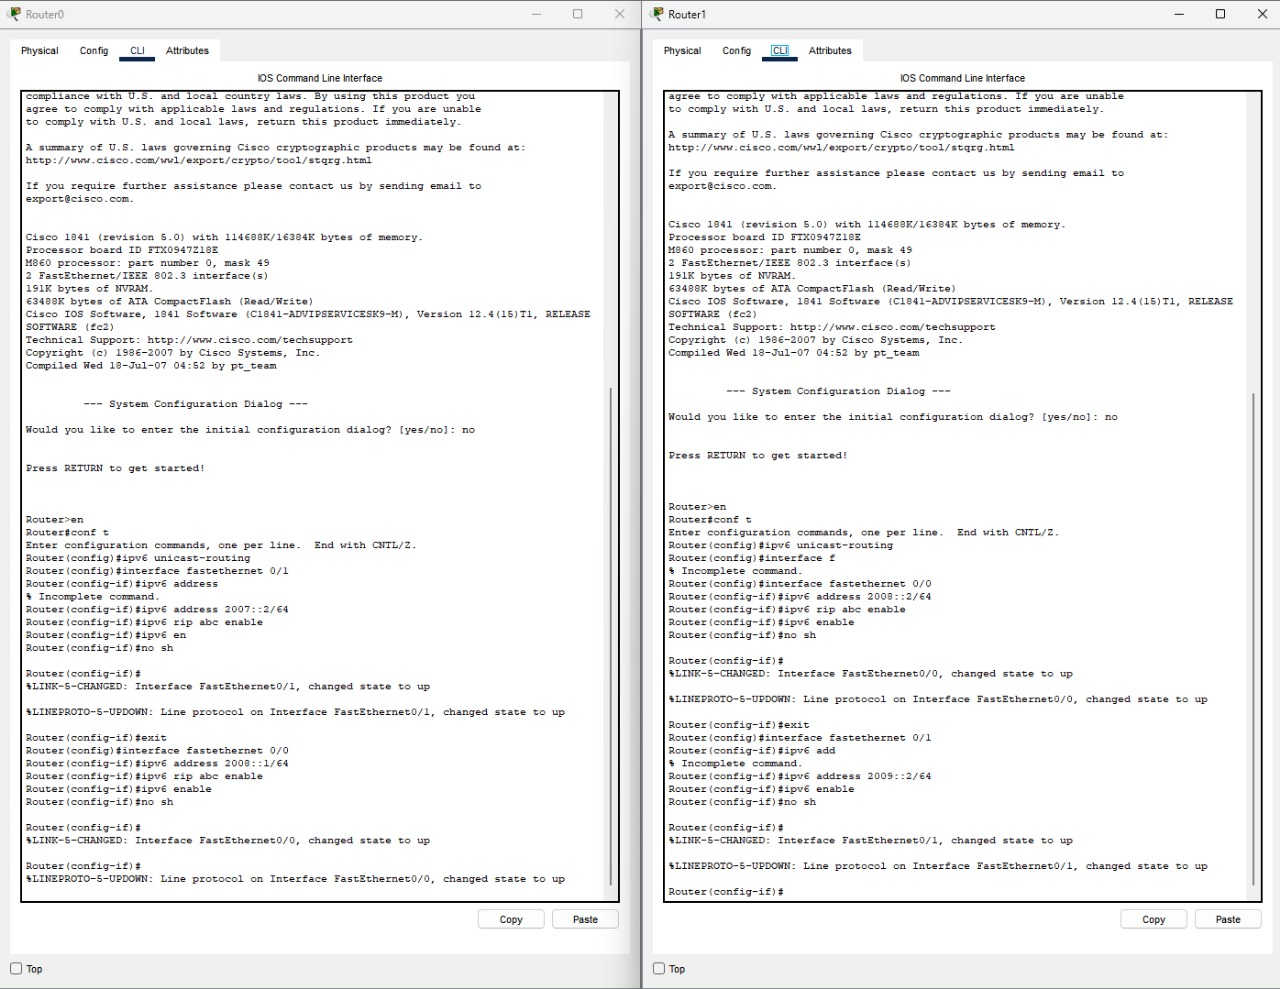
\includegraphics[width=0.48\textwidth]{img/TM7.jpeg}
    \caption{CLI konfigurasi antarr­outer}
    \label{fig:tm7}
\end{figure}

\begin{figure}[H]
    \centering
    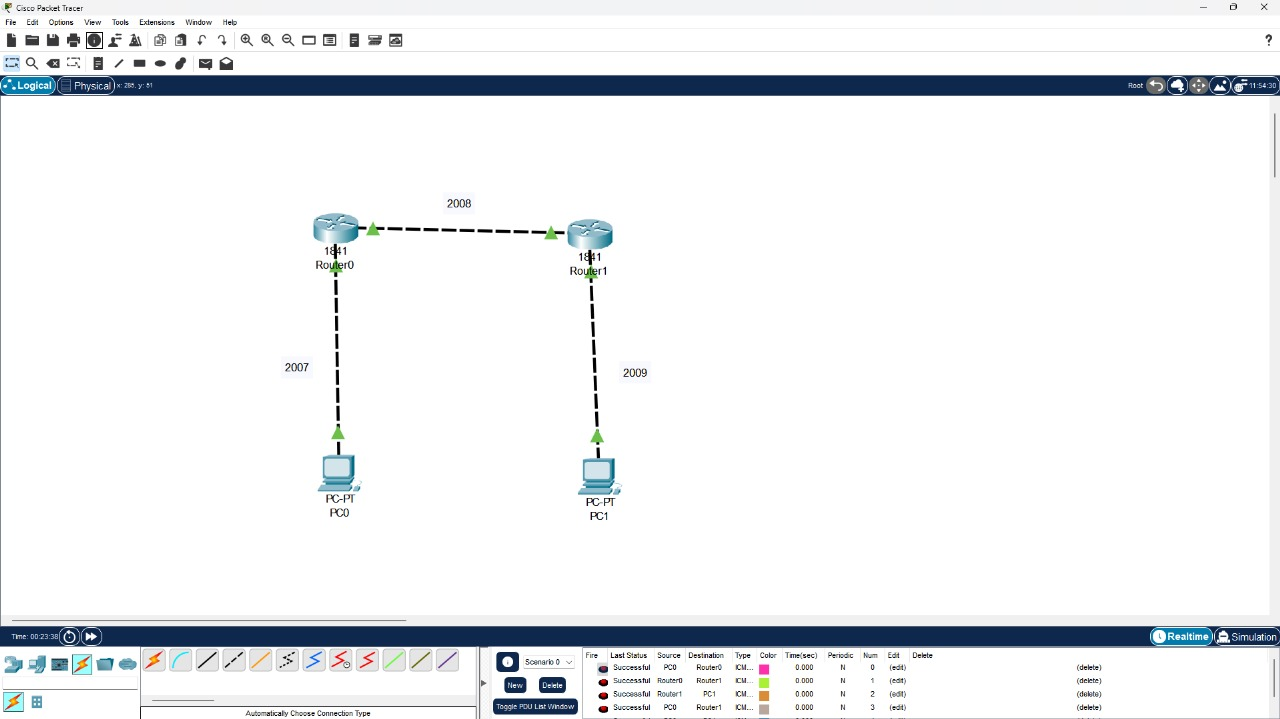
\includegraphics[width=0.48\textwidth]{img/TM8.jpeg}
    \caption{Topologi terkoneksi dan uji \textit{ping}}
    \label{fig:tm8}
\end{figure}

\newpage
\section{Lampiran}

\subsection{Dokumentasi Saat Praktikum}

\begin{figure}[H]
    \centering
    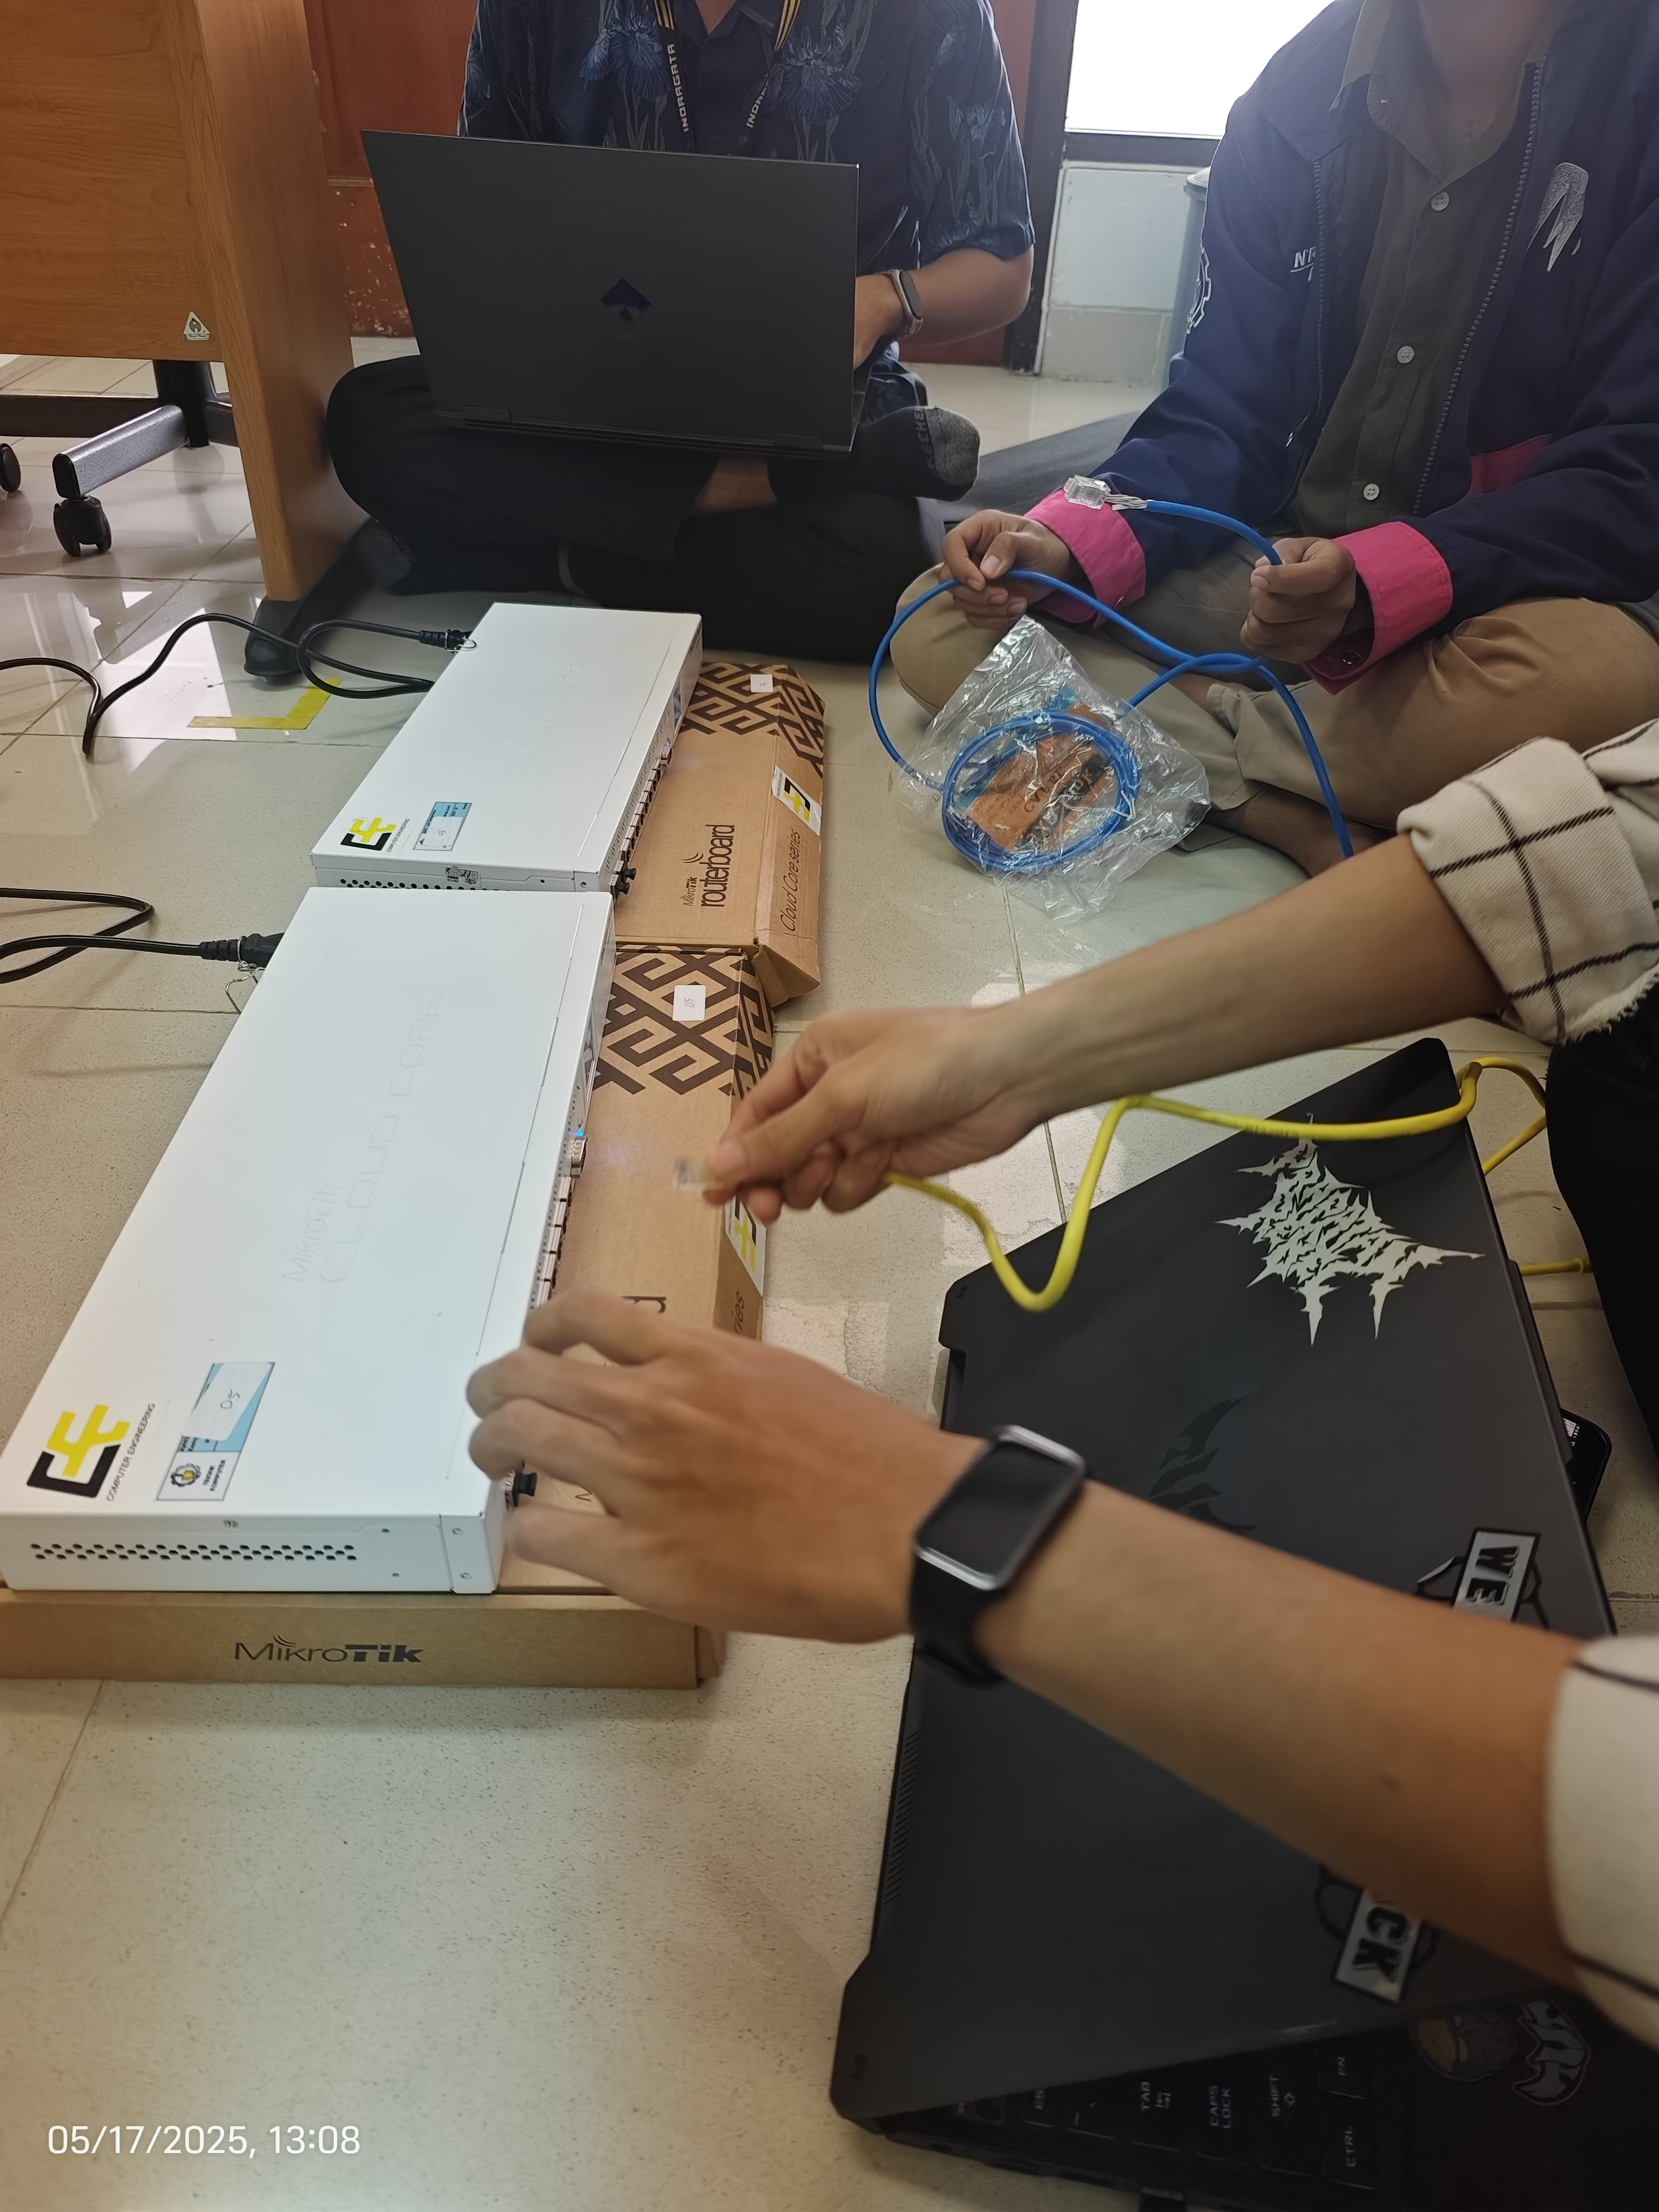
\includegraphics[width=0.48\textwidth]{img/Lampiran1.jpeg}
    \caption{Praktikan menyusun kabel}
    \label{fig:lmp1}
\end{figure}

\begin{figure}[H]
    \centering
    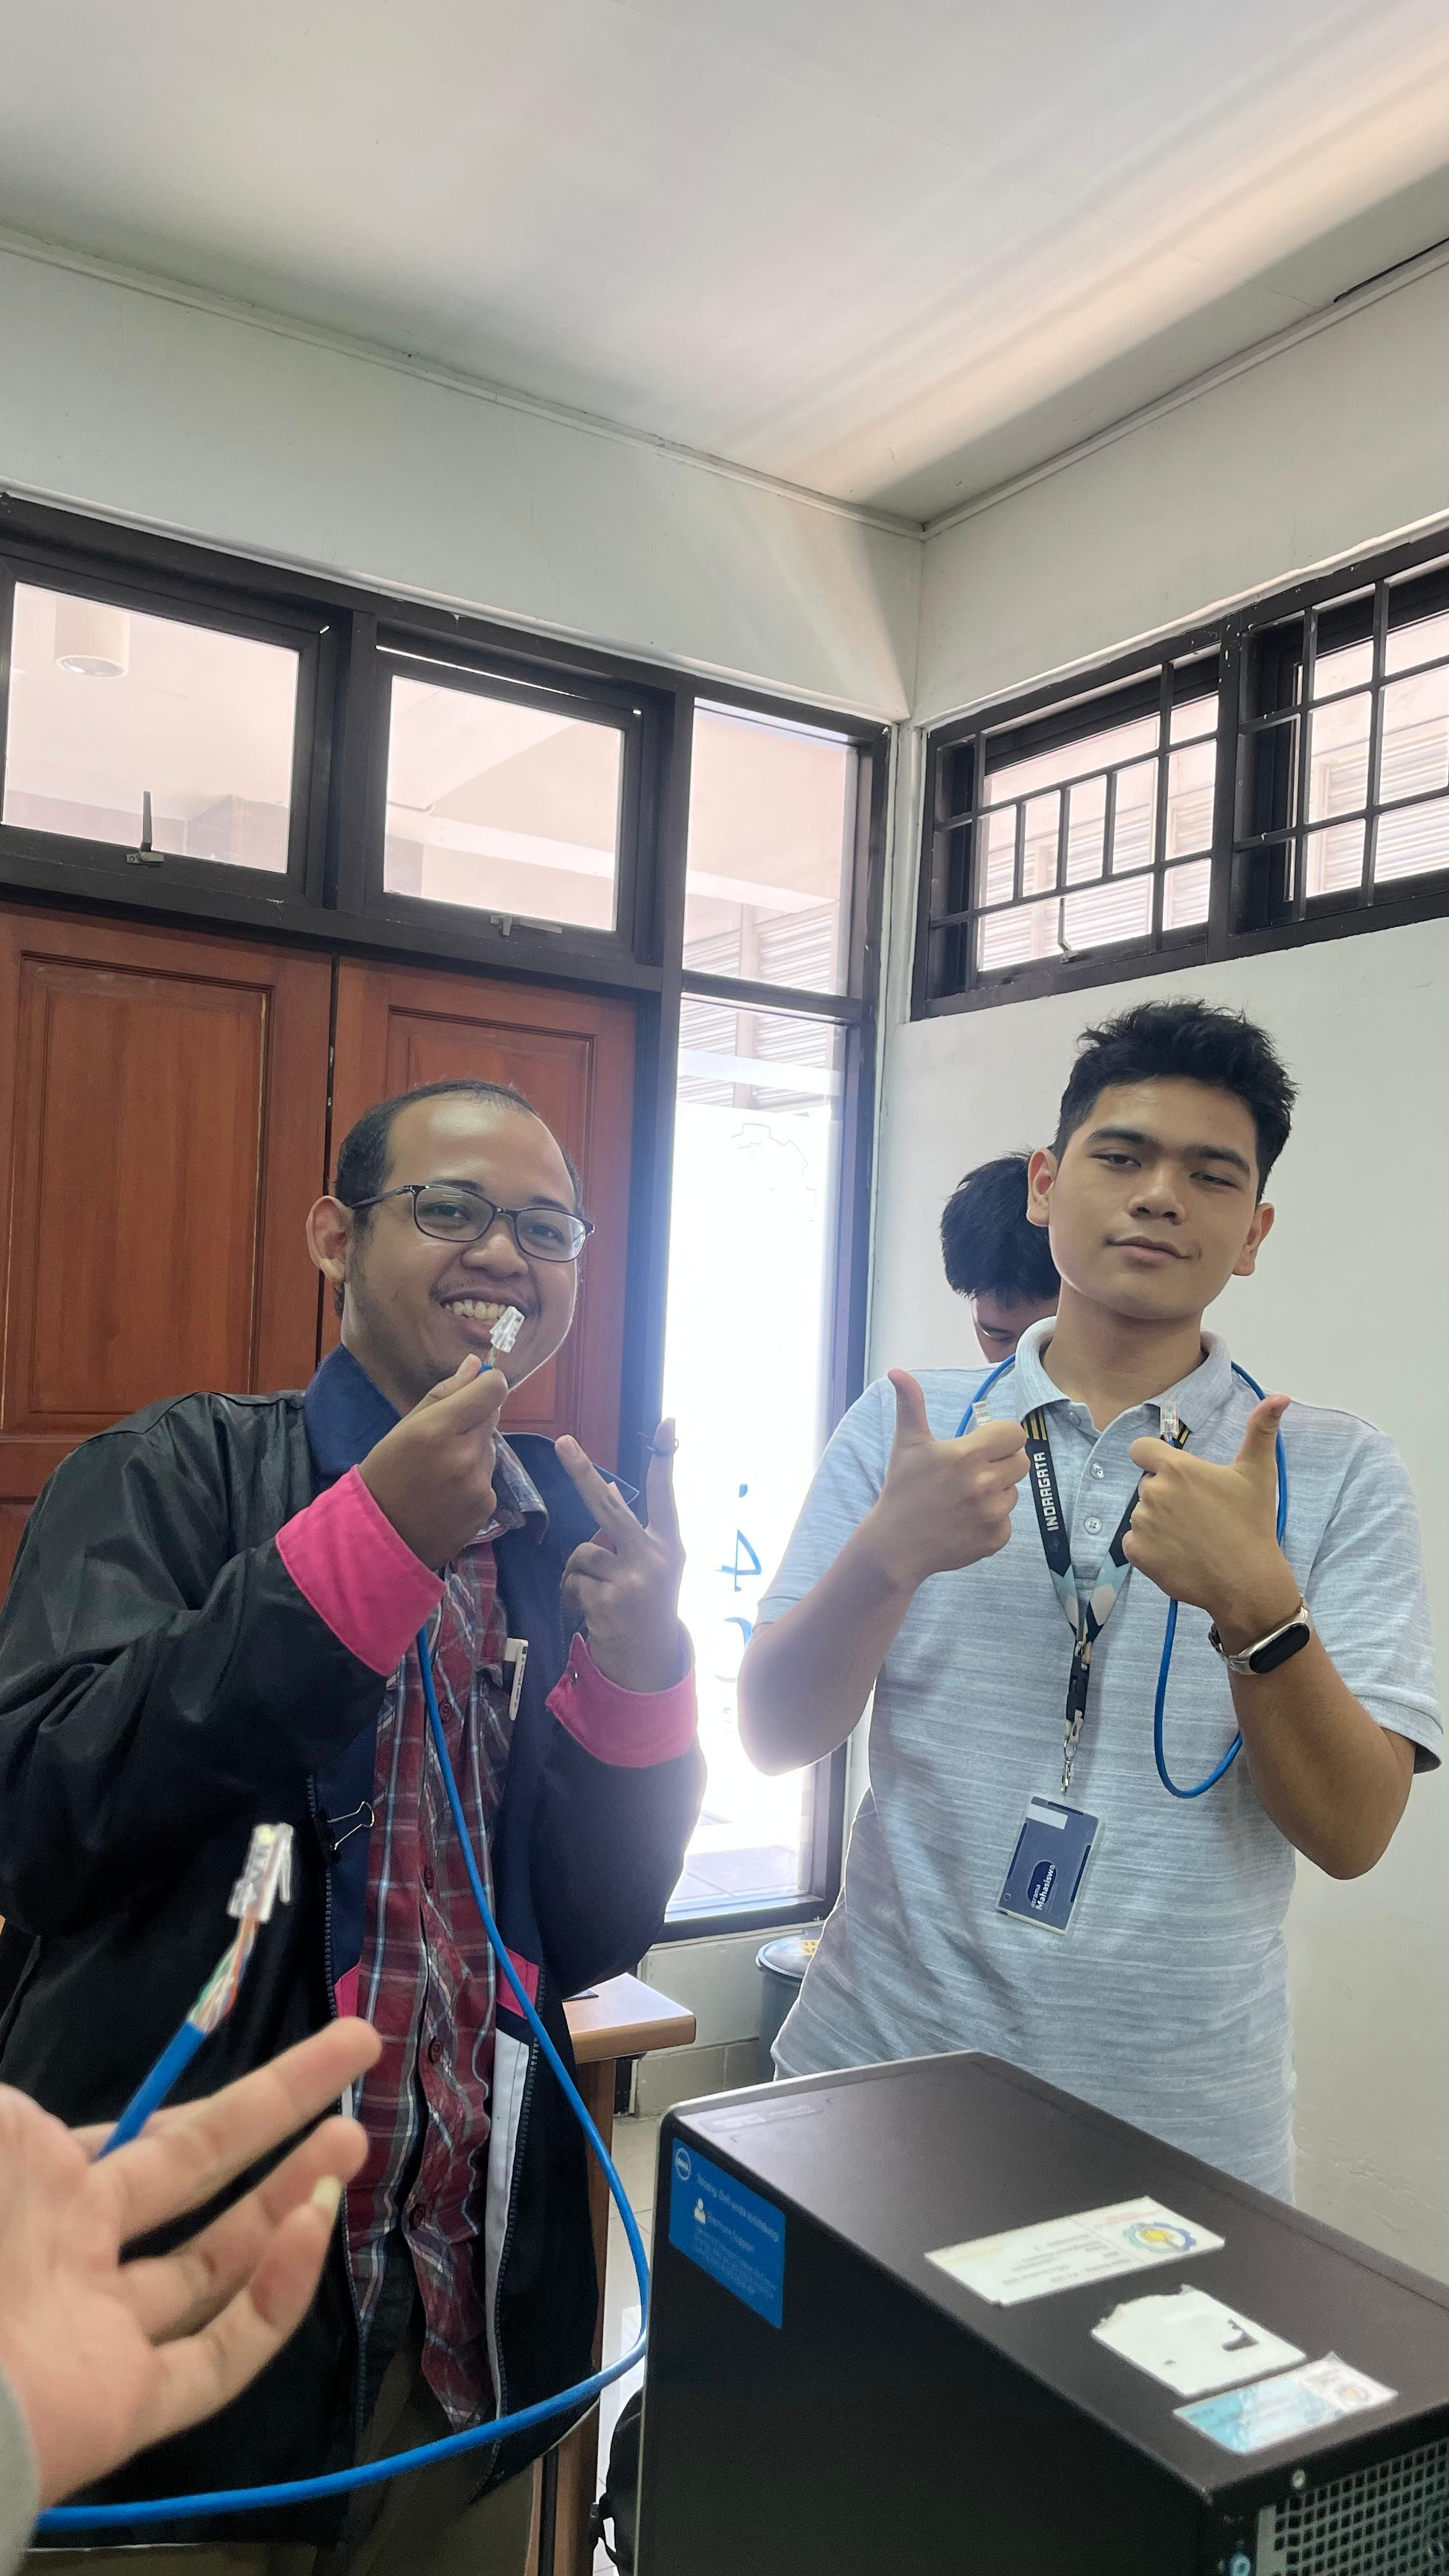
\includegraphics[width=0.48\textwidth]{img/Lampiran2.jpeg}
    \caption{Praktikan saat praktikum}
    \label{fig:lmp2}
\end{figure}



